%==============================================================================
%  Understanding Is Not Observable
%  Shared Convention Makes Communication Possible and Its Measurement Impossible
%
%  MAIN PAPER.  Supersedes and absorbs both earlier manuscripts:
%    - paper/   "A Theory of Computational Coupling Between Intelligent Systems"
%    - paper2/  "Understanding Is Not Observable" (v0.1.0)
%  Both are archived; this file is the single authoritative manuscript.
%
%  Single-column academic article (standard LaTeX `article` template).
%  Build:  ./build.sh        (pdflatex -> bibtex -> pdflatex x2)
%==============================================================================

\documentclass[11pt,a4paper]{article}

%------------------------------- Page geometry -------------------------------
\usepackage[margin=1in]{geometry}
\usepackage{setspace}
\setstretch{1.06}

%--------------------------------- Encoding ----------------------------------
\usepackage[T1]{fontenc}
\usepackage[utf8]{inputenc}
\usepackage{lmodern}
\usepackage{microtype}
\usepackage[british]{babel}

%--------------------------------- Mathematics -------------------------------
\usepackage{amsmath,amssymb,amsthm}
\usepackage{bm}

%--------------------------------- Structure ---------------------------------
\usepackage{authblk}
\usepackage{enumitem}
\usepackage{booktabs}
\usepackage{array}
\usepackage{threeparttable}
\usepackage{graphicx}
\usepackage[font=small,labelfont=bf,width=0.92\textwidth]{caption}
\usepackage{titlesec}
\usepackage{fancyhdr}
\usepackage[title]{appendix}
\usepackage[htt]{hyphenat}      % permit hyphenation inside \texttt{}
\usepackage{tikz}
\usetikzlibrary{arrows.meta, positioning, calc}

%--------------------------------- References --------------------------------
\usepackage[numbers,sort&compress]{natbib}
\bibliographystyle{plainnat}

%--------------------------------- Hyperlinks --------------------------------
\usepackage[colorlinks=true,
            linkcolor=blue!45!black,
            citecolor=blue!45!black,
            urlcolor=blue!45!black,
            breaklinks=true]{hyperref}
\usepackage[nameinlink,capitalise]{cleveref}
\crefname{assumption}{Assumption}{Assumptions}
\Crefname{assumption}{Assumption}{Assumptions}
\crefrangelabelformat{assumption}{#3#1#4--#5#2#6}
\crefname{proposition}{Proposition}{Propositions}
\Crefname{proposition}{Proposition}{Propositions}
\crefname{corollary}{Corollary}{Corollaries}
\Crefname{corollary}{Corollary}{Corollaries}
\crefname{lemma}{Lemma}{Lemmas}
\Crefname{lemma}{Lemma}{Lemmas}
\crefname{definition}{Definition}{Definitions}
\Crefname{definition}{Definition}{Definitions}
\crefname{remark}{Remark}{Remarks}
\Crefname{remark}{Remark}{Remarks}
\crefname{question}{Open Question}{Open Questions}
\Crefname{question}{Open Question}{Open Questions}
\crefrangelabelformat{question}{#3#1#4--#5#2#6}

%--------------------------------- Theorems ----------------------------------
% Shared numbering across all result environments, via aliascnt so that
% cleveref names each reference by its own type rather than "Theorem".
\usepackage{aliascnt}

\theoremstyle{plain}
\newtheorem{theorem}{Theorem}

\newaliascnt{proposition}{theorem}
\newtheorem{proposition}[proposition]{Proposition}
\aliascntresetthe{proposition}

\newaliascnt{corollary}{theorem}
\newtheorem{corollary}[corollary]{Corollary}
\aliascntresetthe{corollary}

\newaliascnt{lemma}{theorem}
\newtheorem{lemma}[lemma]{Lemma}
\aliascntresetthe{lemma}

\theoremstyle{definition}
\newaliascnt{definition}{theorem}
\newtheorem{definition}[definition]{Definition}
\aliascntresetthe{definition}

\newtheorem{assumption}{Assumption}
\renewcommand{\theassumption}{A\arabic{assumption}}
\newtheorem{question}{Open Question}

\theoremstyle{remark}
\newaliascnt{remark}{theorem}
\newtheorem{remark}[remark]{Remark}
\aliascntresetthe{remark}

%--------------------------------- Macros ------------------------------------
\newcommand{\Fc}{\mathcal{F}}
\newcommand{\Dy}{\mathcal{D}}
\newcommand{\dvar}{\mathrm{d}}
\newcommand{\dop}{\mathrm{do}}
\newcommand{\indep}{\perp\!\!\!\perp}
\newcommand{\TE}{\mathrm{TE}}
\newcommand{\Var}{\mathrm{Var}}
\newcommand{\Cov}{\mathrm{Cov}}
\newcommand{\Ex}{\mathbb{E}}
\newcommand{\Real}{\mathbb{R}}
\newcommand{\code}[1]{\texttt{\small #1}}

%--------------------------------- Headers -----------------------------------
\pagestyle{fancy}
\fancyhf{}
\renewcommand{\headrulewidth}{0.4pt}
\lhead{\small\itshape Understanding Is Not Observable}
\rhead{\small\thepage}
\fancypagestyle{plain}{\fancyhf{}\renewcommand{\headrulewidth}{0pt}\rfoot{\small\thepage}}

%--------------------------------- Title block -------------------------------
\title{\vspace{-1.2cm}\bfseries\Large Understanding Is Not Observable\\[6pt]
\large\mdseries Shared Convention Makes Communication Possible\\and Its Measurement Impossible}

\author[]{Ashok Pasala}
\author[]{Snigdha Gorai}
\affil[]{\normalsize VIT-AP University, Amaravati, Andhra Pradesh, India}
\affil[]{\small Correspondence: \href{mailto:ashokashishms@gmail.com}{\texttt{ashokashishms@gmail.com}}}

\date{August 2026}

\begin{document}
\maketitle
\thispagestyle{plain}

%==============================================================================
\begin{abstract}
\noindent
This paper began as an attempt to give brain-to-brain interface research what Shannon gave
telecommunications: a governing quantity to aim at rather than a catalogue of devices to
imitate. We define one --- \emph{coupling capacity}, a directed, interface-supremum
generalisation of channel capacity over state trajectories --- and prove that it saturates at
the smaller of the two systems' effective representational dimensionalities rather than at the
channel rate. We then show that the quantity so defined cannot be measured, and that the
obstruction is not a defect of our formulation but applies to every observational coupling
measure in current use.

Four fields ask whether one system understands another --- artificial intelligence of its
models, neuroscience of interacting brains, comparative cognition of other species,
philosophy of other minds --- and all four answer the same way: observe what passes
between the systems and infer from it. We argue that this cannot work, for two
independent reasons.

First, we prove a non-identifiability result. Any two systems that can communicate must
already share prior convention, and shared convention is a common cause of both what is
transmitted and how the receiver behaves. There therefore exist dyads with \emph{identical}
observational distributions over signals, internal states and behaviour, one genuinely
coupled and one not. No functional of the observational distribution --- mutual
information, transfer entropy, neural synchrony, representational similarity, behavioural
agreement, or conversational performance --- separates them. The very thing that makes
communication possible is what makes it unmeasurable from observation. The construction is
not a knife-edge coincidence: we exhibit an open set of linear--Gaussian dyads with the
same property.

Second, and independently of confounding, we demonstrate with complete ground truth that
coupling measured at the level of \emph{internal states} does not imply coupling at the
level of \emph{behaviour}. In a trained two-agent system where the sender encodes its
private state into the channel at $R^2 = 0.90$ and a linear decoder recovers that state
from the receiver's hidden layer to a reconstruction error of $0.0017$, the receiver
captures approximately $12\%$ of what the information is worth and performs statistically
at the goal-blind optimum. Removing the channel entirely and handing the receiver the
sender's state directly --- infinite bandwidth, zero noise --- changes nothing. We further
find that randomising a signal is a materially more sensitive probe than ablating it, and
that behavioural sensitivity and functional benefit come apart in turn, so interventional
tests must be calibrated against the value of the information rather than against zero.

We then characterise what does suffice. Functional coupling is identified by adjustment
when the shared convention is observed, by instrumental variation --- for which, we note,
ordinary channel noise qualifies, inverting the usual impulse to denoise --- or by direct
intervention. Two things notably do not suffice: temporal precedence, so that transfer
entropy and Granger causality inherit the full force of the negative result despite being
called directional; and observation of the receiver's internal state, which fails the
front-door criterion for structural reasons that no gain in recording resolution or
interpretability precision can repair. We conclude that functional coupling is an
\emph{interventional} quantity sitting one rung above where it is currently measured, and
that this, rather than any deep obscurity in the phenomenon, is why debates about machine
understanding do not resolve. We derive consequences for AI evaluation, mechanistic
interpretability and hyperscanning, note that the framework retrodicts the decade-long
stagnation of brain-to-brain interface bandwidth, and close with the open questions that
would decide the account.
\end{abstract}

\vspace{2pt}
\noindent\textbf{Keywords:} functional coupling; causal identifiability; shared convention;
coupling capacity; transfer entropy; emergent communication; hyperscanning; mechanistic
interpretability; brain-to-brain interfaces; instrumental variables.

\vspace{4pt}
\noindent\rule{\textwidth}{0.4pt}

%==============================================================================
\section{Introduction}\label{sec:intro}

A recurring question appears in several sciences at once, in slightly different dress each
time.

Artificial intelligence asks whether a model understands an instruction, and answers with
benchmarks, preference ratings and dialogue. Neuroscience asks whether two brains in
interaction are coupled, and answers with inter-brain synchrony and directed information.
Comparative cognition asks whether an animal grasps a signal. Developmental psychology asks
it of infants. Philosophy asks it in general, calls it the problem of other minds, and has
historically concluded that it is not empirically tractable.

Each field attacks the question with the same instrument: \emph{watch what passes between
the two systems, and infer understanding from the pattern}. Score the outputs. Measure the
correlation between internal states. Decode one system's content from the other's activity.

This paper argues that the instrument cannot return the answer --- not because measurement
is noisy or the systems are complex, but because the quantity of interest is not a function
of the data being collected. We give two independent arguments, one theoretical and one
empirical, and one remedy.

\paragraph{How we arrived at this claim.}
We did not set out to prove a negative. The work began on the constructive side of the same
question, in brain-to-brain interface research, which occupies today roughly the position
telecommunications occupied before 1948: considerable engineering technique, no governing
quantity that says what a link is for or how well it is doing. \Cref{sec:attempt} states the
quantity we proposed to fill that gap --- \emph{coupling capacity}, a supremum of directed
information over admissible interfaces --- together with a bottleneck theorem showing it is
capped by representational geometry rather than by bandwidth, and the simulation we built to
test it. The programme did not survive its own controls, and it failed in a way that turned
out to generalise far beyond the interface question that motivated it. We report it first
because the rest of the paper is the diagnosis of that failure, and because the failure mode
is, we will argue, shared by four literatures that have not noticed it.

\paragraph{The theoretical argument.}
\Cref{sec:nonid} is an identifiability result with an unusual structure. Ordinary
confounding is a nuisance that careful design can sometimes remove. Here the confounder
cannot be removed, because it is the precondition of the phenomenon. Two systems can only
communicate if they already share a convention governing what signals mean. That shared
convention is a common cause of what the sender emits and how the receiver behaves. Any
observed coherence between them is therefore explicable \emph{either} by the channel doing
work \emph{or} by both parties independently instantiating a convention they already
held --- and no observational statistic separates these. The prerequisite for communication
is the confounder for its measurement.

\paragraph{The empirical argument.}
\Cref{sec:empirical} is independent and does not rely on confounding at all. In a fully
observable artificial system with ground truth over every variable, we exhibit a receiver
whose internal state provably contains the sender's private information and whose behaviour
provably extracts almost none of its value. State-level coupling is at ceiling; functional
coupling is at floor. Since essentially all neural coupling measures and all decoding-based
interpretability findings are state-level, this is a direct demonstration that such measures
do not license behavioural conclusions.

\paragraph{The remedy.}
\Cref{sec:remedy} follows from the diagnosis. If functional coupling is not identified by
observation, it must be identified by intervention: ablate or randomise the channel and
measure whether behaviour changes. What survives the removal of a signal is what the signal
was doing. Everything else is fluency. We add one requirement that the interventional
literature does not usually impose --- that the effect be reported on the scale of the value
of the information, not against a null --- because our own data show sensitivity and benefit
dissociating.

\subsection{Contributions}\label{sec:contributions}

\begin{enumerate}[leftmargin=1.6em, itemsep=3pt]
    \item A formal target for interface research --- coupling capacity (\cref{def:cc}) and an
    effective-dimensionality bottleneck theorem (\cref{thm:bottleneck}) --- stated in full,
    together with an explicit account of why its empirical validation does not support it and
    why the quantity it bounds is not recoverable from observation (\cref{sec:attempt}). The
    theorem stands as a statement about what a bandwidth-limited interface can drive; the
    measurement programme built on it does not.

    \item A non-identifiability theorem for functional coupling under shared convention
    (\cref{thm:nonid}), with the observation that the confounder is constitutive rather than
    incidental, and a linear--Gaussian family (\cref{prop:generic}) showing the construction
    occupies an open set of parameters rather than a measure-zero coincidence.

    \item A matching positive result (\cref{thm:id}) giving three sufficient conditions for
    identification, together with two sharp negatives: temporal-precedence measures such as
    transfer entropy do \emph{not} escape the theorem (\cref{prop:time}), and receiver-side
    measurement does not rescue it via the front-door criterion (\cref{prop:frontdoor}).

    \item A demonstrated instrumental-variable route --- exogenous channel noise as an
    instrument (\cref{rem:noise}) --- validated on a controlled construction and then
    \emph{falsified as a general recipe} on a trained system we did not design for it, with
    the mechanism of failure diagnosed rather than merely reported.

    \item A ground-truth demonstration that state-level and behaviour-level coupling
    dissociate, including an infinite-bandwidth control in which the channel is deleted and
    the sender's private state handed to the receiver directly (\cref{prop:gap},
    \cref{sec:empirical}).

    \item A reporting statistic --- the captured share of the value of information
    (\cref{def:rho}) --- with an estimator, a confidence procedure and a checklist, motivated
    by our finding that a receiver can be measurably perturbed by a signal while deriving no
    benefit from it.

    \item An account of why the gap arises: coupling is a jointly held convention, an
    attractor of shared history, which cannot be established unilaterally
    (\cref{sec:why}); and a consequent prediction of hysteresis.

    \item Consequences for AI evaluation, interpretability and hyperscanning
    (\cref{sec:implications}), and a retrodiction: the framework explains the decade-long
    flatness of brain-to-brain interface throughput against large hardware gains, and
    locates the error in the bandwidth argument that motivates such interfaces
    (\cref{sec:bbi}).

    \item An explicit register of open questions (\cref{sec:open}), each stated so that a
    determinate answer would change the account.
\end{enumerate}

\subsection{Scope, and what we do not claim}\label{sec:scope}

We are not claiming to have solved semantics, and we do not use ``understanding'' in a
phenomenal or philosophical sense. Throughout, \emph{functional coupling} names a specific
causal quantity: the extent to which one system's signal changes what another system does.
Our claim is that this modest, operational quantity --- not consciousness, not meaning in
any rich sense --- is already unidentifiable by the methods four fields currently use, and
that this is enough to invalidate a substantial body of inference.

Three further boundaries should be stated at the outset rather than left to
\cref{sec:limits}. (i) \Cref{thm:nonid} is a statement about what observational data cannot
determine \emph{absent further assumptions}; it is not a claim that coupling can never be
estimated, and \cref{thm:id} says exactly when it can. (ii) \Cref{prop:gap} is an existence
proof on one trained system; it establishes that the dissociation is possible and shows a
mechanism by which it arises, not that it is prevalent. (iii) The interventional protocol of
\cref{sec:remedy} has been applied to the artificial system reported here and not yet to
human--AI or hyperscanning data; \cref{sec:open} states those as the principal outstanding
obligations, with designs.

\subsection{Roadmap}
\Cref{sec:attempt} states the coupling-capacity programme, its bottleneck theorem, and the
controls that ended it; a reader interested only in the paper's standing claims may begin at
\cref{sec:setup}. \Cref{sec:setup} fixes notation and the causal object of interest.
\Cref{sec:nonid} proves non-identifiability. \Cref{sec:identification} characterises when identification is
recoverable and when it is not. \Cref{sec:empirical} reports the state--behaviour
dissociation, \cref{sec:why} explains it, and \cref{sec:remedy} gives the measurement
protocol. \Cref{sec:implications} draws consequences for four fields, \cref{sec:related}
positions the argument against prior work, \cref{sec:limits} states how it could be wrong,
and \cref{sec:open} lists what would settle it. Proofs, experimental detail and a
pre-registered protocol for the outstanding human--AI study appear in the appendices.

%==============================================================================
\section{The target we set out to supply}\label{sec:attempt}

Before 1948, telecommunications engineering possessed extensive practical technique but no
rigorous definition of information or of a medium's fundamental capacity. Shannon's
contribution \citep{shannon1948mathematical} was not a device but a measurement theory: it
specified the upper bound on error-free transmission over any noisy medium, and thereby gave
a field a target to aim at rather than a catalogue of gadgets to imitate.

Brain-to-brain interface (BBI) and brain--computer interface research occupies an analogous
position. Considerable ingenuity goes into tokenisation schemes, neural decoders and aligned
embedding spaces \citep{pais2013brain, rao2014direct, jiang2019brainnet, thual2022aligning},
yet two questions have no agreed answer:

\begin{enumerate}[label=(\alph*), leftmargin=1.9em, itemsep=2pt]
    \item What quantity is being optimised across a link between two systems?
    \item What bounds that quantity for two dynamic, non-stationary neural manifolds?
\end{enumerate}

Absent answers, ``success'' is whichever downstream behavioural score a given paper reports,
and results across hardware, species and modality cannot be placed on a common axis. This
section states the quantity we proposed, the one theorem we proved about it, and --- in
\cref{sec:sim,sec:pivot} --- exactly what our validation did and did not establish.

\subsection{Coupling capacity}\label{sec:cc}

Let each system $i$ be characterised by a state space $\mathcal{M}_i$, a manifold carrying an
internal state trajectory $x_i(t)$, together with a self-predictive model $P_i$ that predicts
$x_i(t+\Delta)$ from $x_i(\le t)$. We deliberately do not assume $\mathcal{M}_i$ is shared,
aligned, or even of comparable dimension across systems --- a departure from hyperalignment
approaches, which presuppose a common representational geometry.

An \emph{interface} from $i$ to $j$ is a possibly stochastic map
$g_{i\to j}: x_i(\le t) \mapsto s_{i\to j}(t)$ producing a signal that influences the
subsequent evolution of $x_j$, subject to a bandwidth or structural budget --- a discrete
channel of vocabulary size $K$, a continuous channel of bandwidth $B$, a hardware-constrained
stimulation protocol. Write $\mathcal{G}$ for the admissible set under a given budget. The
directed coupling under $g$ at lag $\Delta$ is the transfer entropy
\citep{schreiber2000measuring, massey1990causality}
\begin{equation}\label{eq:te}
\TE_{i \to j}(\Delta; g) \;=\; I\big(x_i(t)\, ;\, x_j(t+\Delta) \,\big|\, x_j(\le t)\big),
\end{equation}
the reduction in uncertainty about $j$'s future beyond what $j$'s own past supplies. The
explicit lag matters because biological systems exhibit genuine transmission delay and
representational drift, which a lag-free formulation would misattribute to noise.

\begin{definition}[Coupling capacity]\label{def:cc}
The coupling capacity from system $i$ to system $j$ is the supremum of directed coupling over
admissible interfaces,
\begin{equation}
C(i \to j) \;=\; \sup_{g \,\in\, \mathcal{G}} \; \TE_{i \to j}(\Delta; g).
\end{equation}
\end{definition}

This is the dynamical analogue of Shannon capacity: where Shannon's is a supremum over input
distributions of mutual information under a power constraint, coupling capacity is a supremum
over \emph{interface designs} of directed information between coupled dynamical systems. Total
coupling is $C_{\text{total}} = C(i\to j) + C(j\to i)$, with an asymmetry index
\begin{equation}\label{eq:asym}
A \;=\; \frac{C(i \to j) - C(j \to i)}{C(i \to j) + C(j \to i)} \;\in\; [-1, 1],
\end{equation}
predicted to track task-defined role --- leading versus following, speaking versus listening.

\subsection{The dimensional bottleneck}\label{sec:bottleneck}

The programme's substantive claim was that coupling capacity is bounded by representational
geometry rather than by the wire.

\begin{theorem}[Effective-dimensionality bottleneck]\label{thm:bottleneck}
Let systems $i$ and $j$ have effective representational dimensionalities
$d_i = \dim_{\mathrm{eff}}(\mathcal{M}_i)$ and $d_j = \dim_{\mathrm{eff}}(\mathcal{M}_j)$, and
let the interface be a channel of scalar bandwidth $B$ bits per step. Then
$C(i\to j; B)$ is non-decreasing in $B$ and
\begin{equation}\label{eq:bottleneck}
C(i \to j; B) \;\le\; \min\!\big(B,\; \bar{c}\cdot\min(d_i, d_j)\big),
\end{equation}
where $\bar{c}$ is a per-direction capacity in bits per independently drivable dimension per
step. Consequently, as $B \to \infty$ the capacity saturates at
$C^\ast = \bar{c}\cdot\min(d_i, d_j)$, independently of further bandwidth.
\end{theorem}

\begin{proof}
\emph{Bandwidth bound.} The path $x_i(t) \to s_{i\to j}(t) \to x_j(t+\Delta)$ is a Markov
chain, since $x_j$ is influenced by $x_i$ only through the transmitted signal. By the data
processing inequality,
\[
I\big(x_i(t); x_j(t{+}\Delta)\mid x_j(\le t)\big)
\;\le\; I\big(s_{i\to j}(t); x_j(t{+}\Delta)\mid x_j(\le t)\big) \;\le\; B,
\]
the last step because the channel carrying $s_{i\to j}$ has Shannon capacity $B$.

\emph{Dimensional bound.} The exogenous drive enters $x_j$'s update through an injection
operator whose image lies in the tangent space of $\mathcal{M}_j$, of dimension $d_j$; it can
excite at most $d_j$ independent directions. Symmetrically the source can supply at most $d_i$
independent predictive components, so the number of independently couplable directions is
$\min(d_i,d_j)$. Each is a scalar coupled channel whose capacity is bounded by a finite
constant $\bar{c}$ set by that direction's dynamic range relative to the receiver's intrinsic
process noise. Summing over directions gives $C \le \bar{c}\cdot\min(d_i,d_j)$, with no
dependence on $B$.

\emph{Monotonicity.} Enlarging $B$ enlarges $\mathcal{G}$, and a supremum over a larger set
cannot decrease. Taking the minimum of the two bounds and letting $B\to\infty$ gives the
stated saturation.
\end{proof}

\Cref{thm:bottleneck} is, we believe, correct, and we do not withdraw it: it is a statement
about what a bandwidth-limited interface can drive into a receiver of finite effective
dimension, and its proof uses nothing beyond the data processing inequality and a tangent-space
count. Concavity of $C(\cdot;B)$ in $B$ --- the smooth approach to the ceiling --- follows from
a time-sharing argument in the cases we checked; a general proof remains open. What does not
survive is the measurement programme built on top of the theorem, for reasons given in
\cref{sec:pivot}.

\subsection{Three predictions, and what the simulation actually showed}\label{sec:sim}

The theorem and definition yield three falsifiable predictions.

\begin{description}[leftmargin=2.6em, itemsep=3pt, font=\normalfont\bfseries]
    \item[P1 --- Saturation law.] $C(i \to j; B)$ increases monotonically and concavely in
    $B$, saturating at $\bar{c}\cdot\min(d_i,d_j)$ --- that is, at the smaller system's
    \emph{effective} dimensionality rather than at the channel's rate. Falsifier: capacity that
    keeps scaling with bandwidth well past that ceiling.
    \item[P2 --- Self-prediction governs efficiency.] The capacity achieved per unit of
    bandwidth, $C/B$, increases jointly in the two systems' self-predictive accuracies $R_i$ and
    $R_j$: better internal world models extract more coupling from an identical channel.
    \item[P3 --- Asymmetry tracks role.] The asymmetry index \eqref{eq:asym} correlates with an
    externally defined task role across domains.
\end{description}

We tested these in a seeded sandbox of two coupled stationary vector-autoregressive processes
joined by a quantised $B$-bit channel, with the receiver's effective dimensionality, the
coupling gain and the bit budget all set by hand, reporting mean $\pm$ s.d.\ over five seeds
under both a predictive-gain estimator and the model-free Kraskov--St\"ogbauer--Grassberger
$k$-nearest-neighbour estimator \citep{kraskov2004estimating}. All three predictions were
supported. Capacity saturated far below the raw channel limit, with ceilings of $0.81$, $1.63$
and $3.17$ bits/step at $d_{\mathrm{eff}} = 2, 4, 8$, i.e.\ a slope of
$\bar{c}\approx 0.39$ bits per dimension, and the ceiling tracked the hidden rank $r$ rather
than the ambient dimension when a rank-$r$ manifold was embedded in a $16$-dimensional state.
Coupling efficiency $C/B$ rose from $0.21$ to $0.72$ as self-predictive accuracy rose towards
$0.9$ (Pearson $r = 0.94$). The asymmetry index tracked the role parameter from $-0.89$ through
$0$ to $+0.88$ (Pearson $r = 1.00$). The two estimators, one parametric and one geometric,
agreed to within $2\%$ (Pearson $r > 0.99$).

\begin{figure}[t]
\centering
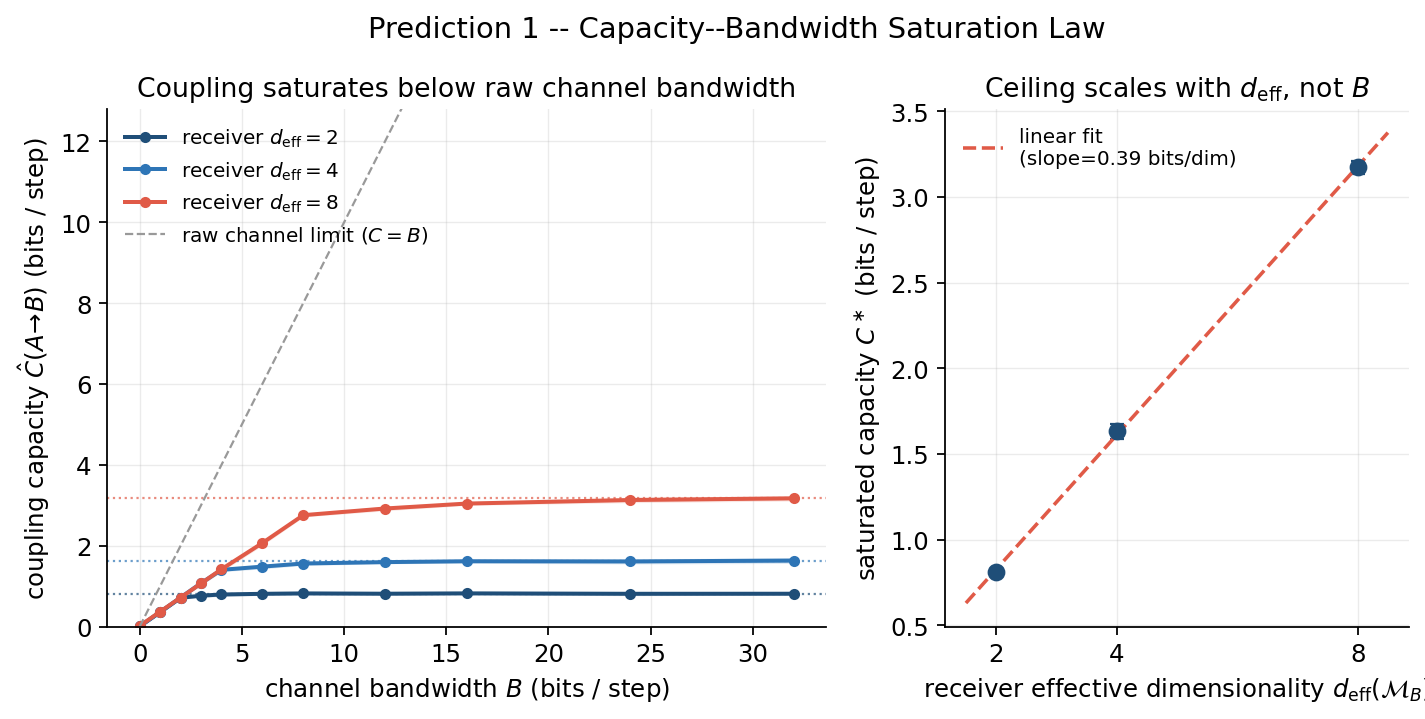
\includegraphics[width=0.98\textwidth]{fig2_capacity_bandwidth_law.png}\\[6pt]
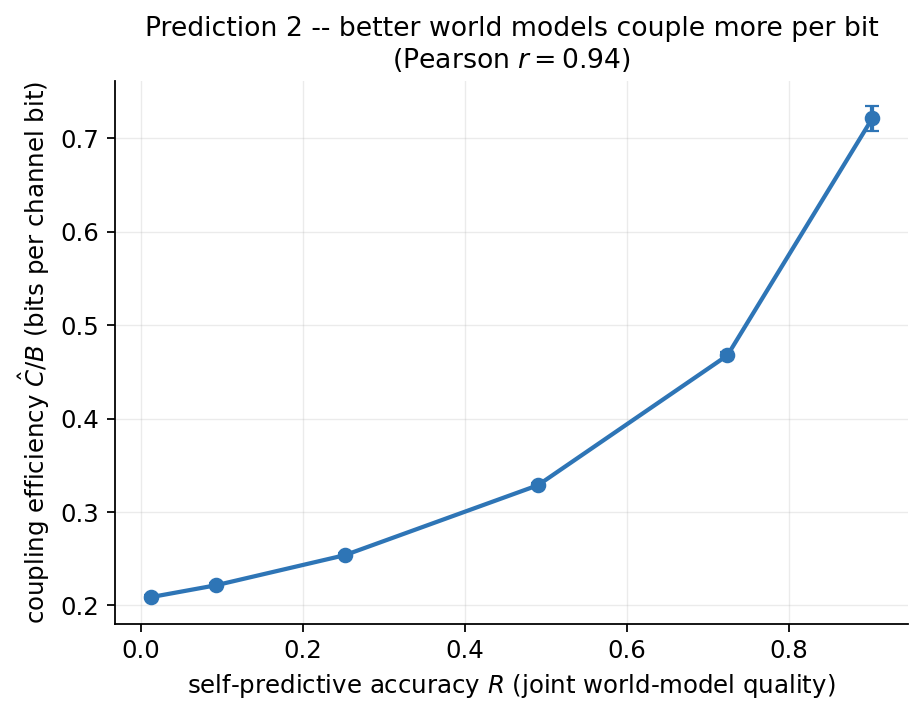
\includegraphics[width=0.44\textwidth]{fig4_selfpredictive_efficiency.png}
\hfill
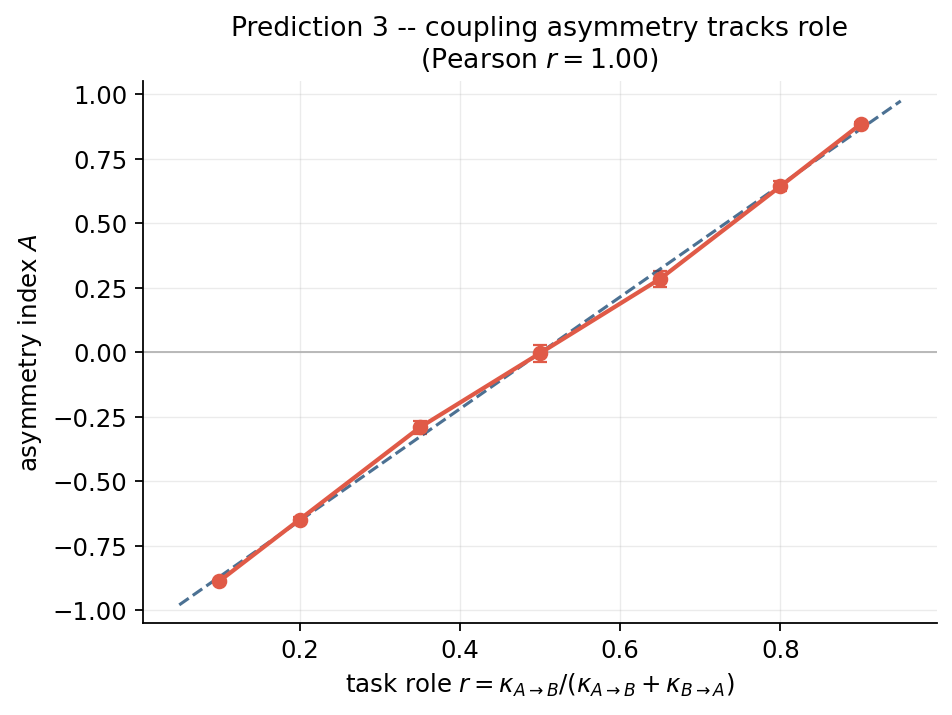
\includegraphics[width=0.44\textwidth]{fig3_asymmetry_index.png}
\caption{The superseded validation. Top: measured capacity against channel bandwidth for three
receiver dimensionalities, saturating far below the raw channel limit (grey dashed), with
ceilings linear in effective dimensionality at slope $\bar{c}\approx0.39$. Bottom left:
coupling efficiency $C/B$ against joint self-predictive accuracy. Bottom right: asymmetry index
against the imposed role parameter. Every panel behaves as \cref{thm:bottleneck} and P1--P3
require. \Cref{sec:sim} explains why this is nonetheless not evidence for the theory: the
quantities being recovered were the ones written into the simulator.}
\label{fig:oldsim}
\end{figure}

\paragraph{What this established.}
Less than it appeared to, and we state the shortfall plainly because the rest of the paper is
about what follows from it.

The simulation satisfies the theory's assumptions by construction: it is linear, Gaussian and
stationary, its manifolds have a dimensionality we chose, and its coupling has a gain we set.
Under P3 in particular, a coupling parameter was imposed on the simulator and then recovered
with $r = 1.00$; that is a demonstration that the estimator inverts the generative model, which
is a property of the estimator, not evidence about the theory. The same reading applies with
less force to P1 and P2. A measurement theory does need to behave correctly where ground truth
is known --- this is a necessary condition --- but we presented it at the time as
confirmation, and it is not.

Two subsequent findings converted that overstatement into a structural problem.

\paragraph{The estimator produced coupling where there was none.}
Carried to a learned interface, the predictive-gain estimator reported a clean monotone
bandwidth--coupling relationship at $r = 0.99$ --- apparently P1 confirmed on a second, harder
system. It was bias: the estimator is an in-sample regression whose bias grows with the ratio of
channel dimension to sample size, and a pure-noise control returned $0.71$ ``bits'' where the
true value was zero. A block-shuffled surrogate correction removed essentially the entire
effect, after which measured coupling sat at the noise floor across bandwidths $1$--$128$. We
return to this in \cref{rem:artefact}, because it is the thesis of this paper occurring at the
level of practice.

\paragraph{The receiver ignored the channel, and then ignored the answer handed to it.}
In the same learned-interface study the sender could be made to encode its private state at
$R^2 = 0.90$ and the receiver's hidden layer made to carry that state at reconstruction error
$0.0017$, with no behavioural consequence whatever; and a receiver given the sender's state
\emph{directly}, with the channel deleted, behaved identically to one given nothing.
\Cref{sec:empirical} reports this in full. Its immediate consequence here is that the bound in
\eqref{eq:bottleneck} was never the binding constraint on that system. \Cref{thm:bottleneck}
is not contradicted --- an unused channel is trivially consistent with any upper bound on what
it could have driven --- but the quantity the programme proposed to maximise turned out not to
be the quantity that governs whether two systems accomplish anything together.

\subsection{Why the programme could not be completed}\label{sec:pivot}

The transfer entropy of \eqref{eq:te} is a functional of the joint observational distribution
of the two trajectories: in the vocabulary of \cref{def:obs} it is a $\Phi$, and coupling
capacity, being a supremum of such functionals over interfaces, is one too. \Cref{thm:nonid}
therefore applies to it directly, and \cref{prop:time} closes the escape that its directionality
appears to offer. Two systems that can communicate at all must already share a convention; that
convention is a common cause of what is sent and how the receiver acts; and no functional of the
observational distribution --- \eqref{eq:te} included --- separates a dyad in which the channel
does the work from one in which it does not.

The programme was thus not defeated by an experimental disappointment that better tuning would
repair. It was aimed at a quantity on the wrong rung of the causal hierarchy
\citep{pearl2009causality}. The remainder of this paper makes that claim precise, shows that it
generalises well beyond interfaces, establishes a second and independent failure that does not
involve confounding at all, and gives the interventional protocol that replaces the programme
described above. \Cref{sec:bbi} returns to brain-to-brain interfaces with the diagnosis in hand,
and finds that it retrodicts the field's most conspicuous anomaly.

%==============================================================================
\section{Formal setup}\label{sec:setup}

\Cref{sec:attempt} defined coupling over state trajectories, which is the natural object when
the question is how much a channel can drive. The question of the rest of this paper is whether
the channel drives anything at all, and for that a coarser object suffices. Consider a dyad
consisting of a sender $A$ and a receiver $B$ exchanging signals over some channel.

\begin{definition}[Dyad]\label{def:dyad}
A dyad is a tuple $\Dy = (Z_A, M, Z_B, U)$ of random variables, where $Z_A$ is the sender's
internal state, $M$ is the signal crossing the channel, $Z_B$ is the receiver's internal
state and $U$ is the receiver's behaviour, together with a structural causal model
specifying how each is generated \citep{pearl2009causality}.
\end{definition}

We are deliberately permissive about what these denote. In hyperscanning, $Z_A$ and $Z_B$ are
neural recordings and $M$ is speech, gesture or gaze. In human--AI interaction, $Z_A$ is the
user's intent, $M$ the prompt, $Z_B$ the model's activations and $U$ its output. In
multi-agent learning they are agent states and messages. The argument is indifferent to
substrate.

One further ingredient is deliberately not part of the tuple, precisely because it is
generally unobserved: a convention-bearing latent $C$ --- the code, language or learned
protocol the dyad already shares, without which $M$ could not function as a signal at all.
\Cref{sec:nonid} introduces it formally; it is flagged here because it is the reason the
tuple above, exhaustive as it looks, does not determine $\Fc$.

\begin{table}[t]
\centering
\small
\begin{tabular}{@{}ll@{}}
\toprule
\textbf{Symbol} & \textbf{Meaning} \\
\midrule
$Z_A$ & sender's internal state (intent, neural state, private observation) \\
$M$   & signal transmitted across the channel \\
$Z_B$ & receiver's internal state (activations, neural recording) \\
$U$   & receiver's behaviour (action, output, response) \\
$C$   & convention-bearing latent shared by the dyad; generally unobserved \\
$N$   & exogenous channel noise, candidate instrument (\cref{rem:noise}) \\
$\Phi$ & an observational coupling measure: a functional of $P(Z_A,M,Z_B,U)$ \\
$\Fc(\Dy)$ & functional coupling of the dyad (\cref{def:fc}) \\
$\dop(\cdot)$ & Pearl's intervention operator \\
$\rho$ & captured share of the value of information (\cref{def:rho}) \\
\bottomrule
\end{tabular}
\caption{Notation used throughout.}
\label{tab:notation}
\end{table}

\begin{definition}[Observational measures]\label{def:obs}
An \emph{observational} coupling measure is any functional $\Phi$ of the joint distribution
$P(Z_A, M, Z_B, U)$ obtained by passive observation of the dyad.
\end{definition}

This class is broad and contains, to our knowledge, every measure currently in use: mutual
information $I(Z_A;Z_B)$ and its lagged variants; transfer entropy $\TE_{A\to B}$
\citep{schreiber2000measuring} and Granger causality \citep{granger1969investigating};
directed information \citep{permuter2009directed}; the coupling capacity of \cref{def:cc};
phase-locking and coherence measures in hyperscanning \citep{montague2002hyperscanning, hasson2010brain}; representational
similarity and cross-subject decoding; behavioural agreement scores; and performance on
conversational benchmarks including the imitation game \citep{turing1950computing}.

\begin{definition}[Functional coupling]\label{def:fc}
The functional coupling of a dyad is the causal dependence of the receiver's behaviour on
the signal:
\[
\Fc(\Dy) > 0 \quad\Longleftrightarrow\quad
\exists\, m, m' : \; P\big(U \mid \dop(M{=}m)\big) \;\neq\; P\big(U \mid \dop(M{=}m')\big).
\]
Where a magnitude is required we take
\[
\Fc(\Dy) \;=\; \sup_{m,m'} \; \mathrm{D}\!\left(P(U \mid \dop(M{=}m)) \,\big\|\, P(U \mid \dop(M{=}m'))\right)
\]
for a divergence $\mathrm{D}$ fixed in advance.
\end{definition}

Functional coupling is thus an interventional quantity by construction: it lives on the
second rung of the causal hierarchy \citep{pearl2009causality}, whereas every measure in
\cref{def:obs} lives on the first. The question this paper addresses is whether it can
nonetheless be recovered from observational data --- whether some clever $\Phi$ identifies
$\Fc$. The answer is no, and the reason is specific to communication.

\subsection{Assumptions}\label{sec:assumptions}

The results below rest on three assumptions, stated separately so that a reader who rejects
one can see exactly which conclusions fall with it.

\begin{assumption}[Convention precedes communication]\label{as:convention}
For $M$ to function as a signal, there exists a latent $C$, established prior to the
exchange under study, such that the receiver's disposition to respond to $M$ is a function of
$C$. Equivalently, the edges $C \to M$ and $C \to U$ (via the receiver's dispositions) are
present in the dyad's causal graph.
\end{assumption}

This is the substantive assumption, and it is the one the paper's negative results depend
on. It is not an empirical hypothesis about particular dyads so much as a restatement of
what it means for a signal to be a signal \citep{lewis1969convention, skyrms2010signals}: a
transmission in a code the receiver does not hold is not a degraded signal, it is not a
signal.

\begin{assumption}[$C$ is not observed]\label{as:unobserved}
The analyst does not record $C$, and no recorded variable is a sufficient adjustment set for
it.
\end{assumption}

\Cref{as:unobserved} is what makes the problem hard rather than merely tedious; when it
fails, \cref{thm:id}(i) applies and identification is restored. \Cref{rem:adjustment}
discusses how often it fails in practice, which is rarely.

\begin{assumption}[Passivity]\label{as:passive}
The analyst observes the dyad without setting $M$, and has no source of variation in $M$
known to be independent of $C$.
\end{assumption}

\Cref{as:passive} defines the observational regime. \Cref{thm:id}(ii) and (iii) are exactly
the two ways of violating it: find such a source of variation, or manufacture one.

%==============================================================================
\section{Non-identifiability under shared convention}\label{sec:nonid}

\subsection{Why the confounder cannot be removed}

Communication requires prior agreement. For a signal to carry information to a receiver, the
receiver must already possess a convention --- learned, evolved, trained or installed ---
that renders the signal actionable (\cref{as:convention}).

This creates an unusual epistemic situation. The shared convention $C$ is a common cause: it
shapes what the sender emits ($C \to M$) and it shapes how the receiver behaves ($C \to U$),
because the receiver's dispositions were formed under the same convention. Observed coherence
between $M$ and $U$ is therefore ambiguous between two explanations that are ordinarily
distinguished by design --- and cannot be here, because eliminating $C$ eliminates the
possibility of communication along with the confound.

\Cref{fig:dags} makes the ambiguity concrete before the theorem states it formally. The two
dyads constructed in the proof below differ only in whether $M$ lies \emph{on} the causal
path from $C$ to $U$ or merely \emph{beside} it. Both produce a message correlated with
behaviour --- in the left dyad because the message causes the behaviour, in the right dyad
only because both are effects of the same shared convention. No inspection of $(C, M, U)$
alone tells these apart; the difference appears only under intervention on $M$.

\begin{figure}[t]
\centering
\begin{tikzpicture}[>=Stealth, thick, node distance=16mm]
  \node (C1) {$C$};
  \node[right=of C1] (M1) {$M$};
  \node[right=of M1] (U1) {$U$};
  \draw[->] (C1) -- (M1);
  \draw[->] (M1) -- (U1) node[midway, above, font=\scriptsize] {causal};
  \node[below=7mm of M1, font=\small] {$\Dy_1$: genuinely coupled};
\end{tikzpicture}
\hspace{18mm}
\begin{tikzpicture}[>=Stealth, thick, node distance=16mm]
  \node (C2) {$C$};
  \node[above right=6mm and 16mm of C2] (M2) {$M$};
  \node[below right=6mm and 16mm of C2] (U2) {$U$};
  \draw[->] (C2) -- (M2);
  \draw[->] (C2) -- (U2);
  \draw[gray, dotted, <->] (M2) to[bend left=15]
        node[midway, above, font=\scriptsize, gray] {correlated, not causal} (U2);
  \node[below=9mm of C2, font=\small] {$\Dy_2$: confounded, uncoupled};
\end{tikzpicture}
\caption{Both dyads induce the identical joint law over $(C,M,U)$ used in the proof of
\cref{thm:nonid}, so every observational functional $\Phi$ agrees on them. On the left, $M$
mediates the only path from $C$ to $U$: intervening on $M$ changes $U$. On the right, $U$
reads off $C$ directly; $M$ and $U$ are statistically associated (dotted) purely through
their common cause, and intervening on $M$ leaves $U$ unchanged. $\Fc$ tracks the solid
causal arrow into $U$, not the association.}
\label{fig:dags}
\end{figure}

\subsection{The result}

\begin{theorem}[Non-identifiability of functional coupling]\label{thm:nonid}
Under \cref{as:convention,as:unobserved,as:passive} there exist dyads $\Dy_1$ and $\Dy_2$
such that
\[
P_1(Z_A, M, Z_B, U) \;=\; P_2(Z_A, M, Z_B, U)
\qquad\text{yet}\qquad
\Fc(\Dy_1) > 0 = \Fc(\Dy_2).
\]
Consequently no observational measure $\Phi$ identifies $\Fc$.
\end{theorem}

\begin{proof}
Let $C \sim \mathrm{Uniform}\{1,\dots,K\}$ with $K \geq 2$ denote a shared convention-bearing
latent: the content the dyad has learned to coordinate on.

\emph{Dyad $\Dy_1$ (genuinely coupled).} The sender's state is $Z_A = C$; it emits $M = C$;
the receiver's state is $Z_B = M$ and its behaviour is $U = M$. Here $B$ reads the channel and
acts on what it reads.

\emph{Dyad $\Dy_2$ (confounded, uncoupled).} The sender's state is $Z_A = C$ and it emits
$M = C$ exactly as before. The receiver, however, has independent access to $C$ through shared
prior context, and sets $Z_B = C$, $U = C$, ignoring $M$ entirely.

Both dyads induce the same observational law: $Z_A = M = Z_B = U$ almost surely, uniform on
$\{1,\dots,K\}$. Hence $P_1 = P_2$ and every functional of the observational distribution
agrees on them. In particular $I(Z_A;Z_B) = I(M;U) = \log K$ in both --- both dyads look
maximally coupled by every available measure, including measures defined on behaviour.

Now intervene. In $\Dy_1$, setting $\dop(M = m')$ yields $U = m'$, so
$P(U \mid \dop(M{=}m))$ varies with $m$ and $\Fc(\Dy_1) > 0$. In $\Dy_2$, setting
$\dop(M = m')$ leaves $U = C$ unchanged, so $P(U \mid \dop(M{=}m))$ is constant in $m$ and
$\Fc(\Dy_2) = 0$.

Since $\Phi$ depends on the dyad only through $P$, and $P_1 = P_2$ while $\Fc_1 \neq \Fc_2$,
no $\Phi$ can equal $\Fc$.
\end{proof}

\begin{remark}
The construction is elementary; that is the point. The mathematical content is standard
confounding. The substantive claim is about \emph{where} it applies: not to a badly designed
study that could be fixed, but to every dyad capable of communicating at all, because shared
convention is a precondition rather than a nuisance. One cannot randomise away the common
cause without destroying the phenomenon.
\end{remark}

\subsection{The construction is not a knife-edge}\label{sec:generic}

A natural first objection is that \cref{thm:nonid} relies on a deterministic, noiseless,
exactly-matched pair, and that generic dyads --- noisy, continuous, not fine-tuned --- would
be separated by observation. They are not. The following exhibits the same phenomenon on an
open set of parameters in the standard linear--Gaussian family, which is also the family in
which the instrumental-variable remedy of \cref{rem:noise} is verified.

\begin{proposition}[Generic observational equivalence]\label{prop:generic}
Let $C \sim \mathcal{N}(0,\sigma_C^2)$ and $N \sim \mathcal{N}(0,\sigma_N^2)$ be independent
with $\sigma_C^2, \sigma_N^2 > 0$, and let $M = C + N$. Define
\[
\Dy_1:\; U = \kappa M + \varepsilon,
\qquad
\Dy_2:\; U = \kappa' C + \varepsilon',
\qquad
\kappa' \;=\; \kappa\,\frac{\sigma_C^2 + \sigma_N^2}{\sigma_C^2},
\]
with $\varepsilon \sim \mathcal{N}(0,\sigma_\varepsilon^2)$ and
$\varepsilon' \sim \mathcal{N}(0,\sigma_{\varepsilon'}^2)$ independent of everything else.
If
\begin{equation}\label{eq:generic-cond}
\sigma_\varepsilon^2 \;>\; \kappa^2\,\frac{(\sigma_C^2+\sigma_N^2)\,\sigma_N^2}{\sigma_C^2},
\end{equation}
then setting
$\sigma_{\varepsilon'}^2 = \sigma_\varepsilon^2 - \kappa^2(\sigma_C^2+\sigma_N^2)\sigma_N^2/\sigma_C^2$
makes the observable joint laws coincide, $P_1(M,U) = P_2(M,U)$, while
$\Fc(\Dy_1) > 0 = \Fc(\Dy_2)$. Since \eqref{eq:generic-cond} is a strict inequality,
the equivalence holds on an open subset of
$(\kappa, \sigma_C^2, \sigma_N^2, \sigma_\varepsilon^2)$-space.
\end{proposition}

\Cref{app:proofs} gives the calculation. Two consequences are worth stating.

First, the observationally identical pair is \emph{stable under perturbation}: the equivalence
does not require exact tuning of $\kappa$, only that \eqref{eq:generic-cond} hold, so it
cannot be dismissed as a measure-zero artefact. Second, the ordinary least-squares regression
of $U$ on $M$ returns $\kappa$ in \emph{both} dyads, even though the true interventional
effect is $\kappa$ in one and $0$ in the other --- which is precisely what the simulation
reported in \cref{rem:noise} finds ($0.800 \pm 0.005$ versus $0.799 \pm 0.019$ at
$\kappa = 0.8$).

\begin{remark}[Why $C$ must be unobserved]
\Cref{prop:generic} matches the law of the observable pair $(M,U)$ and not of $(C,M,U)$; indeed
$\Cov(C,U)$ differs across the two dyads. This is not a weakness of the construction but a
consistency check on it: if $C$ were observed, \cref{thm:id}(i) would identify $\Fc$ by
back-door adjustment, and no observationally equivalent pair could exist. The equivalence and
the identification result are two sides of \cref{as:unobserved}. When internal states $Z_A,
Z_B$ \emph{are} recorded but $C$ is not --- the usual case in neuroimaging and
interpretability --- the burden is carried by \cref{prop:frontdoor} rather than by this
proposition.
\end{remark}

\subsection{Corollaries}

\begin{remark}[The case that matters most]\label{rem:d2}
$\Dy_2$ is not a contrived pathology. It is a compact description of a large language model in
conversation with a person. The model was trained on the recorded output of human convention;
the user is a member of the culture that produced it. Both parties therefore hold $C$
independently, and their exchanges cohere \emph{whether or not} the user's particular signal
is doing causal work. Fluency is exactly what $\Dy_2$ predicts. This is why conversational
impressions of understanding are not merely unreliable but uninformative in principle.
\end{remark}

\begin{corollary}[Invalidity of conversational evaluation]\label{cor:turing}
Any evaluation procedure that scores a system solely on the distribution of exchanged signals
and responses --- the imitation game and its descendants, dialogue benchmarks, human
preference ratings --- is a functional of $P$ and therefore fails to identify $\Fc$. Such
procedures cannot distinguish $\Dy_1$ from $\Dy_2$ at any sample size.
\end{corollary}

\begin{corollary}[Optimisation is indifferent]\label{cor:rlhf}
Training that maximises an observational score $\Phi$ applies pressure that is by construction
identical on $\Dy_1$ and $\Dy_2$. Feedback schemes that rate outputs therefore cannot select
for functional coupling except through whatever correlation happens to hold in the training
distribution. This is not a claim that current systems lack functional coupling; it is the
claim that the training signal does not distinguish, so any such coupling is incidental to the
objective rather than selected by it.
\end{corollary}

%==============================================================================
\section{When identification is possible}\label{sec:identification}

\Cref{thm:nonid} is a negative result about observational data absent further assumptions. It
is not the claim that functional coupling can never be estimated. This section characterises
what suffices --- and, more usefully for practice, what does not. The negative results in
\cref{sec:insufficient} are the ones with consequences for existing literature.

\subsection{Sufficient conditions}

\begin{theorem}[Identification]\label{thm:id}
Functional coupling $\Fc(\Dy)$ is identified if any of the following holds. Informally: you can
see the confounder and adjust for it; you can find something that jitters the message for
reasons unrelated to the convention and use it as leverage; or you can set the message
yourself.
\begin{enumerate}[label=(\roman*), leftmargin=1.9em, itemsep=3pt]
    \item \textbf{Adjustment.} \Cref{as:unobserved} fails: the convention-bearing latent $C$ is
    observed and satisfies the back-door criterion relative to $(M, U)$. Then
    \[
      P\big(U \mid \dop(M{=}m)\big) \;=\; \sum_c P(U \mid M{=}m, C{=}c)\,P(c).
    \]
    \item \textbf{Instrument.} \Cref{as:passive} fails benignly: there exists $N$ with
    $N \to M$, $N \indep C$, and $N$ influencing $U$ only through $M$. Under standard auxiliary
    assumptions --- linearity, or monotonicity in the discrete case
    \citep{angrist1996identification} --- $\Fc$ is point-identified; absent them it is partially
    identified, with informative bounds \citep{balke1997bounds}.
    \item \textbf{Intervention.} \Cref{as:passive} fails by design: the experimenter can set $M$
    directly. Then $\Fc$ is identified by \cref{def:fc}.
\end{enumerate}
\end{theorem}

\begin{proof}
(i) is back-door adjustment and (ii) instrumental-variable identification, both standard
\citep{pearl2009causality, angrist1996identification}; (iii) is immediate from the definition.
\end{proof}

\begin{remark}[On (i): rarely available]\label{rem:adjustment}
Adjustment is the condition one would most like to have and least often does. Convention is
precisely what is implicit, distributed and unarticulated between two parties; a researcher
able to write down $C$ in full has already solved a harder problem than the one at hand.
Proxies exist --- measured familiarity or shared history for human dyads, overlap between a
user's idiom and a model's training distribution for human--AI pairs --- but adjustment on a
proxy yields partial control, not identification, and the residual confounding is of unknown
sign.
\end{remark}

\subsection{Channel noise as an instrument}\label{sec:noise}

\begin{remark}[An underexploited inversion]\label{rem:noise}
The instrumental route is the practically interesting one, because instruments in this setting
are often already present and are currently discarded. \emph{Exogenous channel noise is an
instrument.} Transmission dropout, trial-to-trial jitter, latency variability, hardware
artefact --- any perturbation of the transmitted signal that is independent of the dyad's
shared convention satisfies the requirements of \cref{thm:id}(ii). This inverts the usual
methodological posture: noise in the channel, ordinarily treated as a nuisance to be minimised
or regressed away, is exactly what renders functional coupling estimable without intervening.
Studies that carefully denoise their channel may be discarding their only source of
identification.
\end{remark}

\paragraph{Verification on a controlled construction.}
We instantiate exactly the linear--Gaussian pair of \cref{prop:generic} --- $M = C + N$ with
$N$ exogenous and independent of $C$, and $U$ depending causally on $M$ (coupled) or on $C$
directly with $M$ inert (confounded), calibrated so that $\Cov(M,U)$ is identical across the
two. The naive observational regression of $U$ on $M$ is statistically indistinguishable
between them ($0.800 \pm 0.005$ versus $0.799 \pm 0.019$ across 200 seeds, $n = 2000$ trials
each), exactly as \cref{prop:generic} predicts. The instrumental estimate
$\widehat{\Fc} = \Cov(U,N)/\Cov(M,N)$ recovers $0.800 \pm 0.007$ for the coupled dyad and
$-0.003 \pm 0.034$ for the confounded one, matching each dyad's true interventional effect.
The observational gap between the two dyads is $0.0011$; the instrumented gap is $0.8022$,
against a ground truth of $0.8$.

This holds only once the instrument is strong enough. Sweeping the instrument's strength
$\sigma_N \in \{0.02, 0.1, 0.3, 1.0, 3.0\}$ and recording the first-stage $F$-statistic
alongside each estimate: at $\sigma_N = 0.02$ ($F = 1.6$) the IV estimate is worthless, with a
standard deviation larger than the effect itself; at $\sigma_N = 0.1$ ($F = 20.6$) it begins to
work; by $\sigma_N \ge 0.3$ ($F > 180$) it is essentially exact. The conventional
$F \gtrsim 10$ threshold \citep{stock2005testing} separates the two regimes cleanly here. The
diagnostic must therefore be \emph{reported} alongside the estimate, never assumed.

\begin{figure}[t]
\centering
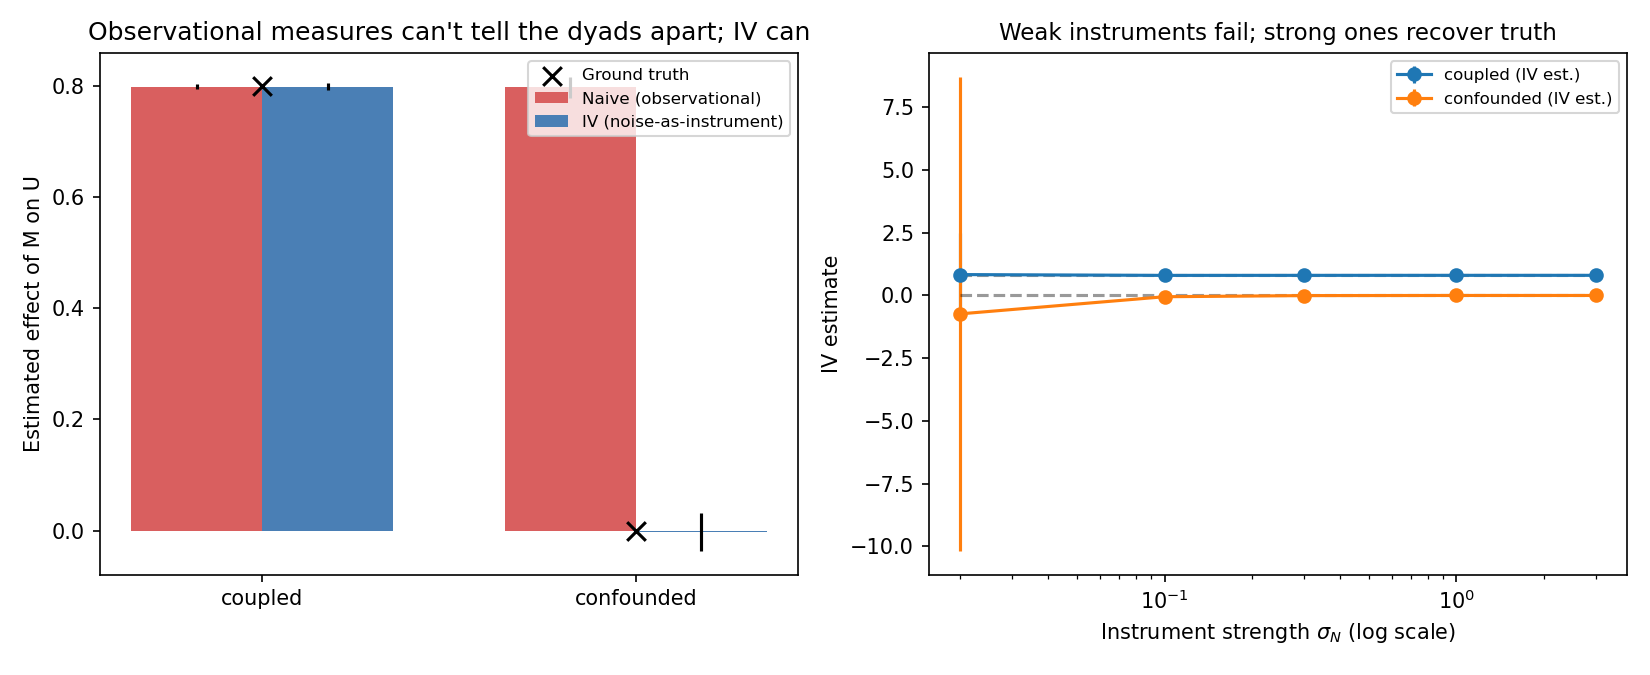
\includegraphics[width=0.95\textwidth]{fig_noise_instrument_toy.png}
\caption{Left: the naive observational regression cannot separate the coupled dyad from the
confounded one --- both return the same estimate, and only the coupled dyad's matches ground
truth, by coincidence. The instrumental estimate recovers each dyad's true value, including the
confounded dyad's true zero. Right: the instrument degrades gracefully as its strength
$\sigma_N$ falls, motivating the first-stage diagnostic rather than an assumed-valid
instrument.}
\label{fig:noise-toy}
\end{figure}

\paragraph{Failure on a system we did not build for it.}
Applying the identical method to the trained system of \cref{sec:empirical} --- using the
discrete channel's own per-step transmission noise as the instrument, over 150 goals $\times$ 20
noise redraws each, 3000 full episode rollouts --- the instrument fails outright: first-stage
$F = 0.2$, and the resulting IV estimate's 95\% confidence interval spans $[-715, 886]$, useless
in either direction.

The failure is itself informative, and we can say why rather than merely that. A variance
decomposition shows that across repeated noise draws for an identical goal the emitted message
barely moves: within-goal variance is $0.3\%$ of total message variance, while across-goal
variance is $99.7\%$. The auxiliary loss that makes this channel informative
($R^2 \approx 0.90$; \cref{sec:empirical}) trains the sender's logits toward confident extremes,
far from the threshold that the channel's own noise perturbs --- so the same optimisation that
produces a usable code simultaneously starves that code's transmission noise of instrumental
relevance.

This is a genuine, checkable boundary condition on \cref{rem:noise}, not a defect in the
controlled demonstration above. It generalises to a warning: well-trained discrete
communication channels are a plausible common source of weak instruments, because optimisation
pushes them towards low-entropy, saturated codes, and that is exactly the regime in which
transmission noise stops being informative about the transmitted symbol --- independently of
whether functional coupling is present. Biological channels (speech, EEG artefact, stimulation
jitter) are not optimised for threshold reliability in this way, so the specific failure mode
may be milder there; but that is a claim to check, not to assume (\cref{q:hyper}).

\begin{figure}[t]
\centering
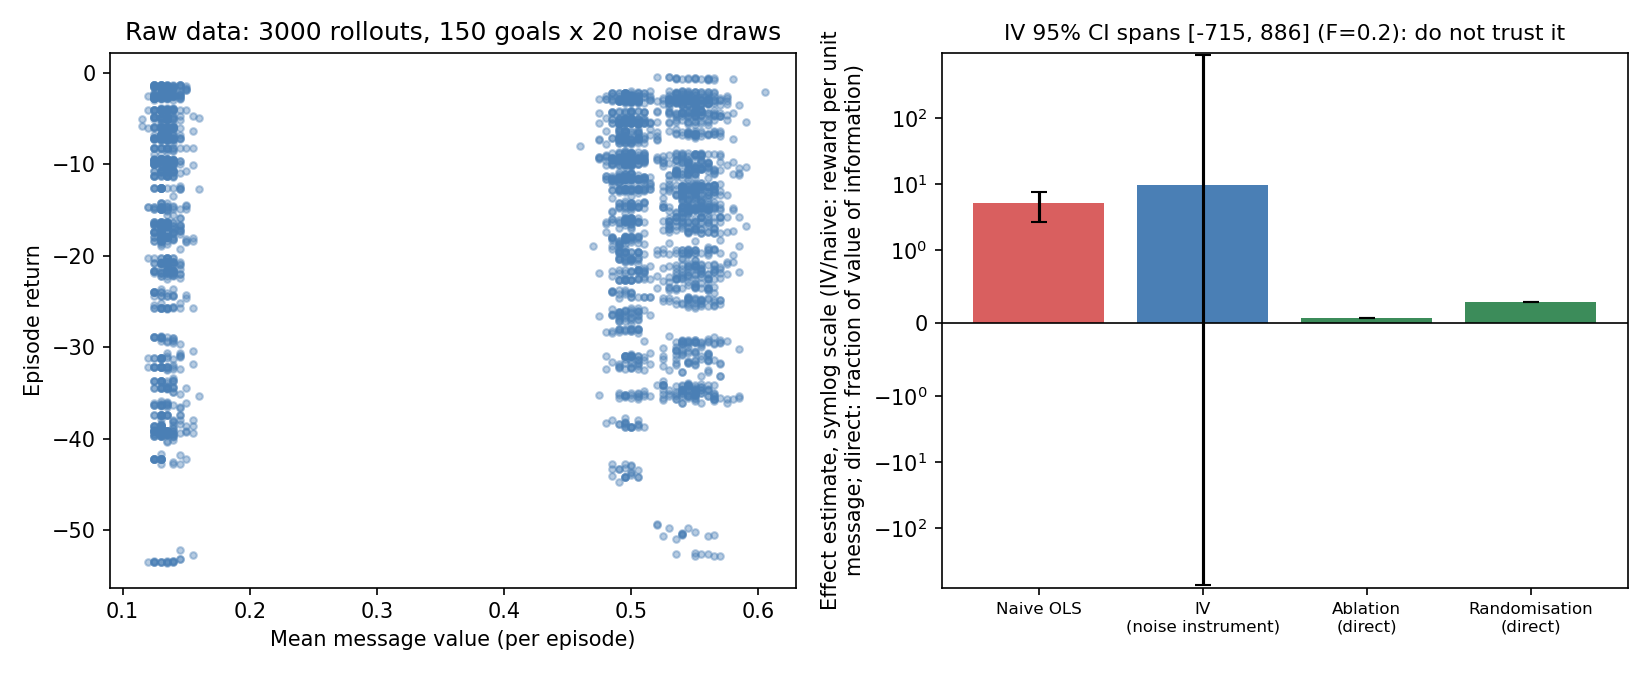
\includegraphics[width=0.95\textwidth]{fig_noise_instrument_stage2.png}
\caption{Left: raw rollouts on the real trained system. Message value clusters by goal rather
than varying smoothly with noise --- visible evidence of the low within-goal variance the text
describes. Right: naive OLS and the IV estimate are both far from the ablation- and
randomisation-based direct estimates of the value of information, and the IV estimate's error
bar is enormous. The first-stage diagnostic ($F=0.2$) correctly flags the estimate as unusable
rather than letting a point estimate mislead.}
\label{fig:noise-stage2}
\end{figure}

\subsection{What does not suffice}\label{sec:insufficient}

\begin{proposition}[Temporal precedence is insufficient]\label{prop:time}
Measures defined by temporal ordering do not identify $\Fc$. Because $C$ precedes both $M$ and
$U$, conditioning on the past of $U$ does not block the back-door path
$M \leftarrow Z_A \leftarrow C \rightarrow U$. Transfer entropy, Granger causality and directed
information therefore remain functionals of the observational distribution and fall under
\cref{thm:nonid} --- as does any supremum of them over interfaces, including the coupling
capacity of \cref{def:cc}.
\end{proposition}

This deserves emphasis because such measures are routinely described as ``directed'' or
``causal,'' and the governing intuition is that respecting temporal order supplies causal
content. It does so only in the absence of a common cause preceding both variables. In dyadic
communication such a common cause is not a hazard to be checked for but a structural guarantee:
without prior shared convention there is no communication to measure. The field's principal
workhorse is thus subject to the theorem in full.

\begin{proposition}[Receiver-side measurement is insufficient]\label{prop:frontdoor}
Observing the receiver's internal state does not restore identification via the front-door
criterion --- Pearl's route for identifying a causal effect through a mediator when the direct
treatment--outcome relationship is itself confounded, which requires no back-door confounding
between treatment and mediator and none between mediator and outcome except what the treatment
already blocks. Consider $Z_B$ as candidate mediator on $M \to Z_B \to U$. Front-door
identification requires (a) no unblocked back-door path from $M$ to $Z_B$, and (b) that every
back-door path from $Z_B$ to $U$ be blocked by $M$. If $C \to Z_B$ and $C \to U$, then
$M \leftarrow Z_A \leftarrow C \rightarrow Z_B$ violates (a), and
$Z_B \leftarrow C \rightarrow U$ --- which conditioning on $M$ does not block --- violates (b).
\end{proposition}

Both edges are present whenever the receiver's internal representations and its behavioural
dispositions were shaped by the same prior convention, which is to say whenever the receiver is
capable of communicating at all.

\begin{corollary}\label{cor:resolution}
Neither higher-resolution neural recording nor finer activation-level interpretability restores
identification. \Cref{prop:frontdoor} concerns causal structure, not measurement precision, and
is therefore invariant to improvements in either.
\end{corollary}

\Cref{cor:resolution} combines with the empirical result of the next section to give
receiver-side measurement a double failure: it targets the wrong node, and it cannot be adjusted
into targeting the right one.

\subsection{When nothing suffices: partial identification}\label{sec:bounds}

A study may satisfy none of \cref{thm:id}'s three conditions and still be worth analysing. Point
identification is not the only useful outcome. Two standard tools apply directly and, to our
knowledge, are not currently used in this literature.

If $U$ is bounded --- as it is whenever behaviour is scored on a finite scale, a fixed reward
range, or a rubric --- then even with no assumptions beyond the observed law, $\Fc$ obeys
nonparametric bounds of the Manski type \citep{manski1990nonparametric}: the interventional
contrast is pinned within an interval whose width is set by the range of $U$ and the support of
$M$. The interval always contains zero under \cref{as:unobserved}, which is \cref{thm:nonid}
restated, but it is not the whole real line, and its width is a reportable measure of how much
the design leaves undetermined.

If a candidate instrument is available but its exclusion restriction is only partially credible
--- the common case for channel noise in a corpus not designed around it --- the Balke--Pearl
bounds \citep{balke1997bounds} give the tightest interval consistent with the observed law and a
discrete instrument, without the monotonicity assumption that point identification requires. We
recommend reporting these bounds rather than an unbounded point estimate whenever the first-stage
diagnostic is marginal, since that is exactly the regime in which our own Stage-2 attempt above
produced a confident-looking number spanning three orders of magnitude.

%==============================================================================
\section{The state--behaviour gap}\label{sec:empirical}

\Cref{thm:nonid} concerns confounding. We now show a second, logically independent failure: even
with no confounding and complete ground truth, coupling measured at the level of internal states
does not imply functional coupling.

\begin{proposition}[State--behaviour gap]\label{prop:gap}
There exist dyads in which $I(M; Z_B)$ is near its maximum while $\Fc$ is negligible relative to
the value of the transmitted information.
\end{proposition}

We establish this constructively, in a system where every variable is observable and the causal
structure is known by construction.

\subsection{System}\label{sec:system}

Two neural-network agents were trained jointly in a referential navigation task (PettingZoo
\code{simple\_speaker\_listener}, \citealp{terry2021pettingzoo}). A \emph{speaker} observes a
private goal --- which of three landmarks the partner must reach --- and cannot move. A
\emph{listener} observes its own position and the landmarks but not the goal, and must navigate.
The environment's fixed vocabulary was bypassed in favour of a learned discrete channel of
tunable width, using a straight-through Gumbel--Sigmoid relaxation so that gradients flow from
the listener's loss into the speaker's message \citep{jang2016categorical, foerster2016learning}.
Agents were trained with policy gradients and an auxiliary reconstruction objective that pressures
the message to carry the goal. \Cref{app:experiment} gives the full configuration.

Three quantities were measured after training, on frozen policies:

\begin{itemize}[leftmargin=1.4em, itemsep=2pt]
    \item \textbf{Encoding fidelity} --- $R^2$ of a regression predicting the emitted message from
    the speaker's private goal. This is a \emph{positive signalling} measure in the sense of
    \citet{lowe2019pitfalls}.
    \item \textbf{Representational uptake} --- reconstruction error of a decoder reading the goal
    from the listener's hidden layer, i.e.\ whether the goal is present and linearly available in
    the receiver's internal state. This is the artificial analogue of cross-subject decoding in
    neuroimaging and of feature discovery in interpretability.
    \item \textbf{Functional coupling} --- the behavioural consequence of the message, estimated by
    intervention, in the two forms of \cref{sec:remedy}. \emph{Ablation} replaces the message with
    zeros. \emph{Randomisation} replaces it with a real, in-distribution message the speaker
    genuinely emitted on a different episode, preserving the message marginal exactly while
    destroying the message--state pairing. Both are direct estimates of \cref{def:fc}; we report
    standardised effects $z$ against the intact condition.
\end{itemize}

\subsection{Result}

\begin{table}[t]
\centering
\small
\begin{threeparttable}
\begin{tabular}{@{}p{0.46\textwidth} c p{0.29\textwidth}@{}}
\toprule
\textbf{Quantity} & \textbf{Measured} & \textbf{Interpretation} \\
\midrule
Encoding fidelity (speaker $\to$ message) & $R^2 = 0.90$ & message carries the goal \\
Representational uptake (message $\to$ receiver state) & recon.\ error $0.0017$ & goal present in receiver \\
Message sensitivity of policy (KL, real vs.\ shuffled) & $0.021$ nats & \\
Own-state sensitivity of policy (KL, reference scale) & $0.686$ nats & ${\sim}33\times$ larger \\
\midrule
Functional coupling --- \emph{ablation} (message zeroed) & $z = +0.50$ & no detectable effect \\
Functional coupling --- \emph{randomisation} (message mispaired) & $z = +1.82$ & small, marginal effect \\
\textbf{Captured share of the value of information, $\hat{\rho}$} & $\mathbf{\approx 0.12}$ & \textbf{at the goal-blind optimum} \\
\bottomrule
\end{tabular}
\begin{tablenotes}[flushleft]\footnotesize
\item Standardised effects $z$ are computed against the intact condition. $\hat{\rho}$ is defined in
\cref{def:rho} and computed from the anchors in \cref{tab:oracle}; it is not distinguishable from
zero at the evaluation sample size.
\end{tablenotes}
\end{threeparttable}
\caption{State-level coupling at ceiling; functional coupling small at best, and yielding no task
benefit.}
\label{tab:gap}
\end{table}

The message demonstrably carries the goal. The goal is demonstrably present in the receiver's
internal representation, recoverable by a linear readout at negligible error. Under ablation,
behaviour is statistically indistinguishable from behaviour with the channel zeroed.

Randomisation, however, is not null: destroying the message--state pairing while preserving the
message marginal costs $2.32$ reward units ($z = +1.82$), against $0.58$ units for outright
ablation ($z = +0.50$). Two conclusions follow, and the second matters more than the first.

\paragraph{Randomisation is the more sensitive instrument.}
It detects a residual behavioural dependence on message content that ablation misses --- roughly a
threefold larger standardised effect on the same trained system. We had predicted this ordering on
theoretical grounds (\cref{sec:remedy}); it is here confirmed empirically. A zeroed channel presents
a constant, easily accommodated input, whereas a mispaired but in-distribution message actively
misleads any receiver retaining sensitivity to content. Practitioners adopting the protocol of
\cref{sec:remedy} should prefer randomisation, and should not read a null ablation result as
establishing zero functional coupling.

\paragraph{But the residual sensitivity does no work.}
The relevant scale is the value of the information itself. In this environment an analytic policy
that uses the goal scores $-8.78$ and the best goal-blind policy scores $-16.88$
(\cref{tab:oracle}), so knowing the goal is worth $8.10$ reward units. The trained receiver scores
$-15.87$: statistically at the goal-blind optimum, capturing $\hat{\rho} \approx 0.12$ of the
available value, and that residual is itself marginal. The receiver's behaviour is faintly
perturbable by the message while extracting essentially none of its value.

This is a sharper statement of the dissociation than a flat null would have been.
\emph{Behavioural sensitivity and functional benefit are themselves distinct.} A receiver can be
measurably influenced by a signal and still derive no advantage from it --- which means that even
an interventional measure must be calibrated against what the information is worth, not merely
tested against zero. We accordingly report $\hat{\rho}$ as the primary quantity
(\cref{def:rho}) and recommend it over a bare significance test.

\subsection{The infinite-bandwidth control}\label{sec:oracle}

A natural objection is that some residual channel imperfection is responsible. We removed the
channel.

In a separate condition the listener was given the speaker's private goal \emph{directly},
concatenated to its own observation --- no encoder, no bottleneck, no discretisation, no noise.
This is the limiting case of a perfect interface, and no physical channel can exceed it.

\begin{table}[t]
\centering
\small
\begin{threeparttable}
\begin{tabular}{@{}lcc@{}}
\toprule
\textbf{Policy} & \textbf{Return} & $\bm{\hat{\rho}}$ \\
\midrule
Analytic expert (uses the goal optimally) & $-8.78 \pm 7.76$ & $1.00$ (anchor) \\
Goal-blind heuristic (hedges to landmark centroid) & $-16.88 \pm 9.84$ & $0.00$ (anchor) \\
Random & $-41.94 \pm 34.84$ & --- \\
\midrule
Trained agent, learned channel & $-15.87$ & $0.12$ \\
\textbf{Trained agent, direct goal access (no channel)} & $\bm{-15.96 \pm 9.70}$ & $\bm{0.11}$ \\
\bottomrule
\end{tabular}
\begin{tablenotes}[flushleft]\footnotesize
\item $\hat{\rho}$ is the captured share of the value of information (\cref{def:rho}), computed
against the expert and goal-blind anchors. Neither trained condition is distinguishable from the
goal-blind anchor.
\end{tablenotes}
\end{threeparttable}
\caption{An agent handed the goal for free converges to the goal-blind optimum.}
\label{tab:oracle}
\end{table}

\begin{figure}[t]
\centering
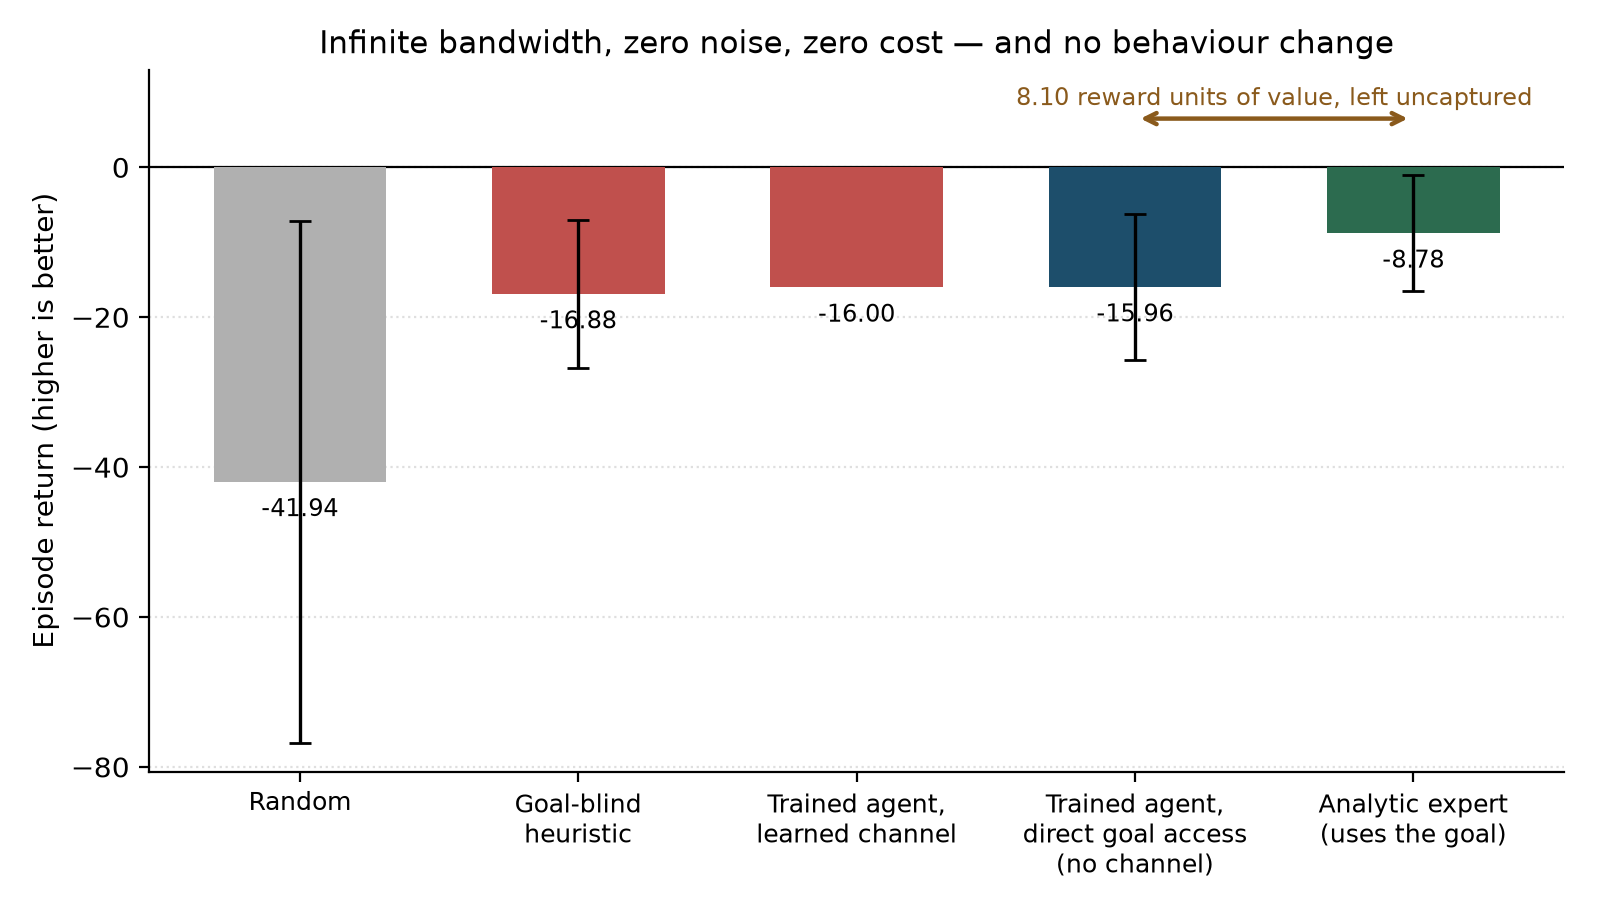
\includegraphics[width=0.82\textwidth]{fig_oracle_control.png}
\caption{Removing the channel entirely and handing the receiver the sender's goal directly does not
move behaviour off the goal-blind optimum, even though an analytic policy shows $8.10$ reward units
are on the table for using it.}
\label{fig:oracle}
\end{figure}

The agent with free, perfect, noiseless access to the information converged to $-15.96$: the score
of the goal-blind heuristic, indistinguishable from agents that received nothing. An analytic policy
that uses the goal achieves roughly twice the return, so the information was both available and
valuable. It was not used, and further training did not change this.

This is the strongest form of the dissociation. The failure is not attributable to bandwidth, noise,
encoding, alignment or capacity, because in this condition none of those exist.

\begin{remark}[A measurement artefact encountered en route]\label{rem:artefact}
During this work an earlier analysis reported a clean monotone relationship between channel
bandwidth and measured transfer entropy ($r = 0.99$), apparently confirming a capacity law. It was
an artefact: the estimator is an in-sample regression whose bias grows with the ratio of channel
dimension to sample size, and a pure-noise control returned $0.71$ ``bits'' of coupling where the
true value was zero. Applying a block-shuffled surrogate correction removed essentially the entire
effect. We report this because it illustrates the paper's thesis at the level of practice:
observational coupling measures can produce confident, well-behaved, theoretically congenial numbers
in the complete absence of coupling. It also stands as a concrete instance of the estimator
fragility documented independently for inter-brain synchrony
\citep{zimmermann2025arbitrary}.
\end{remark}

%==============================================================================
\section{Why the gap exists}\label{sec:why}

The dissociation is not an artefact of weak optimisation, and understanding why illuminates the
general case.

Coupling is not a property of a channel. It is a jointly held convention, and conventions are
attractors of a shared history rather than consequences of contact. Two facts follow.

\paragraph{Coupling cannot be established unilaterally.}
Information has value to a system only if that system already possesses machinery that acts on it;
acquiring that machinery is rewarded only if the information is already being acted upon. Each half
is a precondition for the other, so neither party can move first. Meanwhile there is always a policy
available that ignores the partner and performs moderately well alone --- in our system, hedging
towards the centroid of the candidate landmarks. That policy is reachable immediately, unilaterally,
without coordination. It is found early and it is stable: viewed from inside it, the partner's signal
is worth nothing, so no local gradient points out of it.

Our agents fell into precisely this attractor and never left, with the answer sitting in their own
hidden layer the entire time. We tested a series of independent escapes --- longer training,
learning-rate and gradient-batching sweeps, exploration pressure, an information-aware value baseline,
and auxiliary reconstruction objectives on the sender and on the receiver --- and none produced
behavioural change, because each optimises \emph{within} the basin rather than across its boundary.
\Cref{app:experiment} tabulates them. The last two are the sharpest: they repaired both halves of the
state-level pipeline, raising encoding fidelity to $R^2 = 0.90$ and driving the receiver's
reconstruction error to $0.0017$, and behaviour did not follow.

\paragraph{Coupling should therefore be bistable, and hence historical.}
If coupling is an attractor rather than a channel state, the conditions under which it ignites need
not match the conditions under which an established convention collapses. We predict hysteresis: a
dyad that has already established a convention will sustain coupling under degradation that would
have prevented its formation. If this holds, coupling capacity is not a function of a dyad's present
parameters at all, only of its history --- and cross-sectional measurement of coupling capacity is
ill-posed. This also explains an everyday asymmetry: establishing a shared code, whether a language, a
jargon or a couple's private shorthand, is enormously expensive, while maintaining one is nearly free.
\Cref{q:hysteresis} states the experiment that would decide it.

%==============================================================================
\section{Interventional coupling measurement}\label{sec:remedy}

The diagnosis prescribes the treatment. Functional coupling is defined interventionally, is not
identified observationally, and must therefore be estimated by intervention.

\begin{quote}
\textbf{Protocol.} To establish that a signal is doing work, ablate or randomise it and measure the
change in the receiver's behaviour. Functional coupling is what survives removal of the signal.
\end{quote}

\subsection{Three tiers of intervention}

\begin{enumerate}[leftmargin=1.6em, itemsep=3pt]
    \item \textbf{Ablation.} Replace the signal with a null or constant and measure the behavioural
    difference. Establishes whether the channel carries any functional load.
    \item \textbf{Randomisation.} Replace the signal with one drawn from the same marginal but paired
    with a different underlying state. This is the decisive test against the confound of
    \cref{thm:nonid}: it preserves every surface property of the signal while destroying its
    relationship to the sender's state. A receiver acting on shared prior convention rather than on
    the message is unaffected; a genuinely coupled receiver degrades.
    \item \textbf{Targeted perturbation.} Alter the signal so as to change its meaning under the
    putative convention while holding surface statistics fixed, and check that behaviour tracks the
    altered meaning. Establishes not only that the channel matters but that it matters \emph{in the way
    the convention specifies}.
\end{enumerate}

Randomisation deserves emphasis: it is what defeats $\Dy_2$. Under $\dop(M = m')$ with $m'$ drawn
independently of $C$, the coupled dyad's behaviour changes and the confounded dyad's does not, which is
exactly the discrimination \cref{thm:nonid} shows observation cannot make. \Cref{sec:empirical} confirms
empirically that it is also the more sensitive of the two, detecting residual dependence that ablation
reports as null.

\subsection{A scale: the captured share of the value of information}\label{sec:rho}

An interventional test still requires a \emph{scale}. Establishing that behaviour changes when a signal
is removed does not establish that the signal is doing appreciable work; our own receiver is a case in
point. We therefore propose reporting the effect as a fraction of what the information is worth.

\begin{definition}[Captured share of the value of information]\label{def:rho}
Let $J(\pi)$ be the receiver's expected task performance under policy $\pi$. Let
$\pi^{\star}_{\mathrm{inf}}$ be an optimal policy with access to the sender's state and
$\pi^{\star}_{\mathrm{blind}}$ an optimal policy without it. The \emph{value of information} is
\[
\mathrm{VoI} \;=\; J(\pi^{\star}_{\mathrm{inf}}) - J(\pi^{\star}_{\mathrm{blind}}) \;\ge\; 0,
\]
and the captured share achieved by the observed receiver $\pi$ is
\[
\rho(\pi) \;=\; \frac{J(\pi) - J(\pi^{\star}_{\mathrm{blind}})}{\mathrm{VoI}},
\qquad \rho \in (-\infty, 1].
\]
\end{definition}

Three properties make $\rho$ the right headline number. It is dimensionless, so it is comparable across
tasks with different reward scales. It is zero exactly when the receiver does no better than the best
policy that ignores the signal, which is the substantive null --- rather than ``the intervention changed
nothing,'' which is a weaker and easier-to-satisfy null. And it is bounded above by $1$, so a small
$\rho$ cannot be rescued by a large sample: statistical significance and practical magnitude are
separated by construction.

\paragraph{Estimation.}
$\hat{\rho}$ is a ratio of differences of means and is straightforward to estimate: evaluate each of the
three policies on a common set of $n$ episodes or trials, and obtain a confidence interval for
$\hat{\rho}$ by a nonparametric bootstrap over episodes, resampling the numerator and denominator jointly
so that shared task variation cancels. Where the informed optimum is genuinely unavailable, the
uninformed optimum alone still provides a far more meaningful reference than zero, and the numerator
$J(\pi) - J(\pi^{\star}_{\mathrm{blind}})$ can be reported in task units.

\paragraph{Anchors.}
The two anchors need not be learned. In our environment both are analytic (\cref{tab:oracle}). In
general: $\pi^{\star}_{\mathrm{blind}}$ can be obtained by training or hand-designing a policy that is
architecturally denied the signal, and $\pi^{\star}_{\mathrm{inf}}$ by an oracle policy or a human
ceiling. In discrete evaluation settings the analogues are the base rate of satisfying an unstated
constraint by chance, and the compliance rate of a response constructed with the constraint made
maximally salient (\cref{app:humanai}).

\subsection{Reporting checklist}\label{sec:checklist}

We suggest that any claim of coupling --- between agents, between brains, or between a user and a model
--- report the following. Each item corresponds to a failure documented in this paper.

\begin{enumerate}[leftmargin=1.6em, itemsep=2pt]
    \item The intervention used, from the three tiers above; randomisation at minimum
    (\cref{sec:empirical}).
    \item $\hat{\rho}$ with a bootstrap interval, alongside the raw effect (\cref{def:rho}).
    \item Both anchors, and how they were obtained (\cref{tab:oracle}).
    \item For any instrumented estimate, the first-stage $F$-statistic
    (\cref{sec:noise}; \citealp{stock2005testing}), and Balke--Pearl bounds when it is marginal
    (\cref{sec:bounds}).
    \item For any observational coupling statistic, a surrogate or pure-noise control establishing the
    estimator's bias at the sample size used (\cref{rem:artefact}).
    \item An explicit statement of whether $C$ was observed, proxied, or unobserved
    (\cref{as:unobserved}).
\end{enumerate}

%==============================================================================
\section{Implications}\label{sec:implications}

\subsection{Evaluation of AI systems}
By \cref{cor:turing}, conversational and preference-based evaluation cannot identify functional coupling
between a model and a user's intent. This is a structural limitation, not a matter of benchmark quality
or rater training. The prescription is concrete: evaluate by intervention. Perturb the user's signal in
ways that change intent while preserving surface form, and measure whether model behaviour tracks the
change. A system whose outputs are invariant to such perturbations is exhibiting $\Dy_2$ --- coherent,
fluent and uncoupled. \Cref{app:humanai} gives a complete pre-registered design.

We note the practical stake. Apparent and functional coupling produce identical behaviour \emph{within}
the distribution on which apparent coupling was established, and divergent behaviour outside it. Our
receiver looked unremarkable --- it scored what every other agent scored --- until the situation actually
required the signal, at which point it failed completely. On this account a familiar deployment pattern,
in which systems pass extensive evaluation and then fail in the field, is not a symptom of insufficient
testing but of testing a quantity that does not determine the one that matters.

\subsection{Mechanistic interpretability}
A claim that a model represents some quantity is a statement about decodability from internal state ---
precisely the measure that read $0.0017$ in \cref{tab:gap} while behaviour read effectively zero. Presence
of a feature in a representation licenses nothing about its causal role. The field's causal methods ---
activation patching, causal scrubbing and related interventions \citep{geiger2021causal} --- are therefore
not refinements of decoding-based analysis but the only valid form of the claim. Our result is a clean
existence proof of a feature that is fully present, linearly recoverable and behaviourally inert.

\Cref{cor:resolution} sharpens this into a claim about the field's trajectory. Because the obstruction is
structural, it is not relieved by better probes, larger probing datasets or finer-grained feature
decomposition: a decoding result of arbitrarily high fidelity still licenses no behavioural conclusion.
Progress on decoding accuracy and progress on causal warrant are therefore orthogonal, and effort spent on
the former should not be scored as progress on the latter.

Neuroscience reached a structurally identical conclusion earlier and with a different vocabulary.
\citet{grootswagers2018finding} show with MEG that category information is broadly decodable across visual
cortex while only a subset of it predicts trial-by-trial categorisation behaviour, and the motor literature
has built a mature framework around exactly this distinction, in which a large fraction of population
activity occupies an output-null subspace that cancels at the behavioural readout
\citep{kaufman2014cortical}. That these fields converged independently on the same distinction is evidence
that the gap in \cref{tab:gap} is a general property of layered systems rather than a quirk of our
training setup.

\subsection{Hyperscanning and inter-brain coupling}\label{sec:hyperscanning}
Inter-brain synchrony and directed-information measures are observational, state-level, and applied to
dyads that share both a task and a culture --- that is, a large common cause. Three of our results bear on
this simultaneously, and their conjunction is unusually restrictive. \Cref{thm:nonid} applies directly.
\Cref{prop:time} closes the most natural escape: transfer entropy and Granger causality are the field's
standard instruments precisely because they are directional, but directionality obtained from temporal
ordering does not survive a common cause that precedes both series, and shared convention is exactly such a
cause. \Cref{prop:frontdoor} closes the second: recording more of the receiving brain, at higher resolution,
does not help, because the failure is structural rather than one of measurement precision. And
\cref{prop:gap} adds that even were confounding absent, the quantity being measured is at the wrong node.
Reported inter-brain coupling therefore establishes that two brains' states covary; it does not establish
that either brain's behaviour depends on the other's signal.

The field has independently been moving in a compatible direction, which sharpens rather than weakens the
point. \citet{varlet2024measuring} show that inter-brain synchrony has low sensitivity to whether two people
are actually processing the same information, and propose cross-brain representational analysis as a
replacement; \citet{markus2024hyperscanning} name the directionality problem explicitly and propose dyadic
neurofeedback, Granger causality and structural equation modelling as remedies; and
\citet{zimmermann2025arbitrary} show that arbitrary preprocessing choices skew synchrony estimates
substantially. Our results imply that the first two of \citeauthor{markus2024hyperscanning}'s three
remedies are statistical and therefore remain under \cref{thm:nonid} and \cref{prop:time}, while the
third --- real-time neurofeedback --- is genuinely interventional and is the one to pursue. The commonly used
pseudo-pair control is a step in the same direction but controls for the shared \emph{stimulus} rather than
for the coupling channel itself, and so does not reach $\Dy_2$.

There is also a constructive path that requires no new experiments. By \cref{rem:noise}, exogenous
variability in the transmitted signal --- momentary occlusion, acoustic interference, dropped words, latency
--- is an instrument, provided it is independent of the pair's shared history. Existing hyperscanning
corpora contain such variation and typically treat it as noise to be cleaned. Recovering it and using it as
an instrument is, to our knowledge, an unexploited route to interventional conclusions from
already-collected observational data --- subject to the first-stage diagnostic that our own Stage-2 attempt
failed (\cref{sec:noise}). We further suggest that inter-brain studies adopt signal randomisation as a
standard control, and note a testable consequence: on a fixed task with fixed instrumentation, measured
coupling should track the pair's \emph{prior shared convention} --- strangers below acquaintances below
long-term partners --- and that effect should exceed any channel-quality variable.

\subsection{Brain-to-brain interfaces}\label{sec:bbi}

Direct neural interfaces are motivated by a bandwidth argument, and its premise is well supported. Language
is a narrow, serial channel. Across seventeen languages spanning nine families, conversational speech
converges on an information rate near $39$ bits/s, syllable-rate differences being compensated almost
exactly by differences in information per syllable \citep{coupe2019languages}; the throughput of deliberate
human behaviour more generally has been estimated at roughly $10$ bits/s, some eight orders of magnitude
below the raw capacity of the sensory periphery \citep{zheng2024slowness}. The inference usually drawn is
that the mouth and the ear are the binding constraint on what two minds can accomplish together --- that
cognition is fast and parallel while its expression is slow and serial, and that a cortical link bypassing
articulation and audition would let brains exchange at the rate at which they compute.

The present account grants the premise and rejects the inference. The rate limit is real and is not what
binds. \Cref{sec:oracle}'s infinite-bandwidth control is this hypothesis tested in the only setting where it
can be tested cleanly: we removed the channel entirely and delivered the sender's private state to the
receiver directly, noiselessly, at no cost --- the limit that no physical interface can exceed --- and
behaviour did not move. Capacity was never the quantity in short supply. A pair that does not share a
convention gains nothing from a wider channel, because the gain from widening a channel is bounded by the
amount of the signal the receiver was going to act on, and that amount was approximately zero.

The empirical record on real brain-to-brain systems agrees. The framework retrodicts a standing anomaly, and
the anomaly is documented rather than asserted. \citet{rao2014direct} (2014; 64-channel EEG sender, one TMS
coil, three pairs) transmitted $0.25$--$0.81$ bits/trial. \citet{jiang2019brainnet} (2019; a real-time,
three-person, two-sender architecture, the field's most technically advanced system) transmitted $0.336$
bits/trial for its best sender --- \emph{less} than Rao's best pair five years earlier, despite strictly more
sophisticated hardware and with only a single electrode actually used for decoding out of the 8- and
32-channel systems available. The authors state this themselves: ``From the first human BBI to BrainNet, the
level of information complexity has remained binary\ldots [and] this low bit rate required a disproportionate
amount of technical hardware and setup'' \citep{jiang2019brainnet}. An independent systematic review of the
2013--2020 literature \citep{nam2021prisma} reports the same pattern across the full set of published
studies: methodological diversification (EEG, intracortical microelectrodes, focused ultrasound,
optogenetics; TMS, direct cortical stimulation) without a corresponding rise in bits transmitted, concluding
that mutual information ``has been limited to mostly binary information transfer'' throughout.

On a channel-centric account this is unexplained, and worsens with better hardware rather than improving. On
the present account it is forced: in every such study the convention is installed from outside, in advance,
by ordinary language --- the participant is \emph{told} that a phosphene means ``rotate,'' or the meaning is
fixed by the experimenter's choice of stimulation site. Throughput is therefore bounded not by hardware but
by how much convention can be pre-installed by talking to a subject beforehand. That bound is low and does not
move when the hardware improves; if anything, coordinating a second sender in BrainNet added
convention-installation overhead without adding transmitted content.

This converts into a design claim rather than only a retrodiction. If throughput is bounded by how much
convention can be installed in advance, the way to raise it is to make convention formation part of the
interface instead of a precondition the experimenter supplies verbally beforehand: bidirectional,
closed-loop, and trained across sessions, so that the pair acquires a code neither party held at the outset.
\Cref{sec:why} argues that this is a joint exploration problem and therefore expensive --- neither side can
construct the code unilaterally, which is one reason a child spends years acquiring the conventions of a
first language rather than minutes acquiring its channel. The prediction is that a direct interface does not
avoid that cost; it relocates it into a code for which neither brain has any prior, and better electrodes do
not pay it. \Cref{q:bbi} states the corresponding falsifier.

%==============================================================================
\section{Related work}\label{sec:related}

The components of this argument exist; the synthesis and the identifiability claim, to our knowledge, do not.

\paragraph{Foundations.}
\citet{shannon1948mathematical} explicitly excluded semantics from the engineering problem, a simplification
that was safe while receivers executed protocols fixed in advance and fails once both ends must acquire their
protocol. \citet{pearl2009causality} supplies the ladder on which we locate functional coupling.
\citet{searle1980minds} argued that syntactic competence does not constitute understanding but offered no
test; our contribution can be read as supplying an operational criterion and explaining why conversational
tests could never have provided one. \citet{lewis1969convention} formalised convention;
\citet{harnad1990symbol} posed symbol grounding; \citet{skyrms2010signals} derived meaning from signalling
games.

\paragraph{Directed information and its use between systems.}
\citet{schreiber2000measuring} introduced transfer entropy for model-free asymmetric
dependence between time series and \citet{massey1990causality} formalised directed information
for systems with feedback; \citet{kraskov2004estimating} supply the $k$-nearest-neighbour
estimators used as a model-free cross-check in \cref{sec:sim}. These are the tools from which
\cref{def:cc} was assembled, and \cref{prop:time} is our statement of what they cannot do
between two systems that share a convention. On the interface side,
\citet{pais2013brain, rao2014direct} and \citet{jiang2019brainnet} established physical
feasibility of direct neural links under severe bandwidth constraints;
\citet{thual2022aligning} align functional cortical geometries across subjects by optimal
transport, and \citet{nakamura2024unsupervised} perform zero-shot representation transfer with
hyperspherical embeddings. On our reading, alignment is a technique for raising the quantity in
\cref{def:cc}, not for identifying $\Fc$, and \cref{sec:bbi} argues that the constraint these
systems face is not the one they are engineered against. \citet{friston2015active} model
communication as mutual free-energy minimisation and \citet{hasson2010speaker} document
speaker--listener neural coupling; both motivate why coupled systems synchronise without
supplying a criterion that separates $\Dy_1$ from $\Dy_2$. Self-supervised neural encoders
--- LaBraM \citep{jiang2024labram}, BrainLM \citep{caro2024brainlm}, MindEye2
\citep{scotti2024mindeye2} --- are the state extractors on which a biological instantiation of
these measures would be built, and by \cref{cor:resolution} their improvement does not change
the identifiability situation.

\paragraph{Nearest formal neighbour.}
\citet{kolchinsky2018semantic} define semantic information as information with causal relevance to a system's
viability. Like us, they locate meaning in causal consequence rather than correlation. Unlike us, they do not
address identifiability from observational data or the constitutive role of shared convention as confounder,
and their formalism is monadic --- one system's information about its environment --- rather than dyadic,
which is the structural reason it does not already reach the coupling question we ask. Their contribution is a
definition; ours is an impossibility result about recovering a quantity of that kind from observation.

\paragraph{Emergent communication.}
\citet{lowe2019pitfalls} distinguish positive signalling from positive listening and warn that the former can
be high while the latter is absent --- a distinction we rediscovered empirically before encountering their
terminology, and which \cref{tab:gap} instantiates with ground truth. Their matrix-communication-game
experiments give an independent replication in a different environment: positive signalling (their Speaker
Consistency, $0.19$--$0.54$ across game sizes) coexists with causal influence at the floor, message removal
leaving action-prediction accuracy essentially unchanged. They trace this to an architectural confound ---
shared hidden layers between action and communication heads induce spurious signalling correlations even with
untrained communication parameters. Our diagnostic chain rules out that mechanism for our system (separate
networks, an auxiliary loss raising encoding fidelity to $R^2 = 0.90$, and a listener reconstruction head
decoding the goal at error $0.0017$) and the dissociation persists regardless --- the same symptom via a
different route, which is why we read their result as a second instance of the phenomenon rather than an
explanation of ours. They frame the finding as a metric pitfall with a practical remedy (measure causal
influence, use several estimators); we argue no estimator escapes it without intervention.
\citet{eccles2019biases} introduce explicit biases to induce both signalling and listening, motivated by the
joint-exploration failure \cref{sec:why} describes; \citet{foerster2016learning} address the same obstacle
architecturally.

\paragraph{Decodable but unused.}
The distinction between information that is present and information that is used is well established within
single systems: \citet{grootswagers2018finding} give a direct human-neuroscience instance, and
\citet{kaufman2014cortical} give the mature theoretical vocabulary (output-null versus output-potent
subspaces). Our contribution is to carry the distinction \emph{across} systems, where it interacts with the
convention confounder, and to show that no observational measure recovers it.

\paragraph{Hyperscanning methodology.}
\citet{varlet2024measuring} argue that inter-brain synchrony is insensitive to information alignment and
propose representational analyses instead; \citet{markus2024hyperscanning} frame the problem as one of
directionality; \citet{zimmermann2025arbitrary} document estimator fragility. These converge on distrust of
raw synchrony from three different directions. None frames the problem as non-identifiability, and none
proposes channel ablation or randomisation, which is where our account differs.

\paragraph{Interpretability.}
Interpretability's causal turn \citep{geiger2021causal} already reflects awareness that decoding is
insufficient; we supply an argument for why intervention is necessary rather than merely preferable, and, via
\cref{cor:resolution}, why the necessity does not diminish as probes improve.

%==============================================================================
\section{Limitations and falsification}\label{sec:limits}

We state the ways this could be wrong, in order of severity.

\paragraph{The superseded programme is reported, not defended.}
\Cref{sec:attempt} states the coupling-capacity formalism and \cref{thm:bottleneck} because
they are the origin of the argument and because we take the theorem to be correct as a bound on
what a bandwidth-limited interface can drive. Its empirical support is nonetheless weak in the
specific way \cref{sec:sim} sets out, and the quantity it bounds is exactly the quantity
\cref{thm:nonid} shows to be unidentifiable. A reader assessing the paper's positive claims
should weigh \cref{sec:nonid,sec:identification,sec:empirical,sec:remedy}; \cref{sec:attempt}
is included for the record, and because the failure it describes is what the rest of the paper
explains. Readers of the earlier manuscript should treat its headline validation claims as
withdrawn in the form in which they were stated there.

\paragraph{The assumption set may be narrowable further.}
\Cref{thm:id} gives three sufficient conditions and \cref{prop:time,prop:frontdoor} rule out two tempting
shortcuts, but we do not claim this characterisation is exhaustive. A weaker assumption set that still
identifies $\Fc$ --- particularly one satisfiable in observational hyperscanning corpora, where intervention is
impossible after the fact --- would be a substantial improvement and is where we would look first to
strengthen the paper.

\paragraph{The instrumental route works on the construction built to demonstrate it and fails on the first
system we did not build for it.}
Applying \cref{rem:noise}'s method to the trained speaker--listener, using the channel's own transmission noise
as instrument, gives an unusable estimate (first-stage $F = 0.2$; \cref{sec:noise}) because the auxiliary loss
that makes the channel informative also drives it towards confident, low-noise-sensitivity outputs. This is a
real, diagnosed boundary condition rather than a refutation of the method --- the first-stage check caught it
correctly rather than reporting a misleading point estimate --- but it means the route is not yet shown to work
on any system we did not design to make it work, and whether it survives contact with real, non-optimised
biological channel noise remains open (\cref{q:hyper}).

\paragraph{The empirical demonstration is a single system.}
\Cref{prop:gap} is an existence proof, which is what it needs to be, but it does not establish that the gap is
common in systems of practical interest. If ablation and observational measures agree across a broad range of
real dyads, the correction we prescribe is unnecessary in practice even if valid in principle.

\paragraph{Functional coupling here is small, not provably zero.}
The randomisation effect ($z = +1.82$) is marginal by conventional standards and we do not claim it is null; a
larger evaluation set would sharpen it in one direction or the other. Our claim is the weaker and
better-supported one that the receiver captures almost none of the available value of the information while
every state-level measure is at ceiling. Readers should note that this makes the dissociation a matter of
degree, and that our recommended statistic --- $\hat{\rho}$ --- is what carries the argument, not a significance
test.

\paragraph{Hysteresis is predicted, not shown.}
\Cref{sec:why}'s bistability claim is untested. Coincident onset and collapse thresholds would falsify it and
restore coupling to the status of a state variable of the connection.

\paragraph{The retrodiction rests on few data points.}
\Cref{sec:bbi} cites measured bits/trial from the two best-documented studies (2014 and 2019, five years apart,
throughput flat-to-declining despite more sophisticated hardware) plus an independent systematic review's
qualitative agreement, rather than asserting the pattern from memory. But these are two quantified anchor points
bracketing a decade, not a dense time series, and a general search of the 2021--2026 literature found no further
quantified human-to-human study either confirming or breaking the pattern --- an absence of evidence, not
evidence of the pattern's continuation. A more exhaustive database search, or a new study reporting a materially
higher bit rate, would each bear directly on this claim.

\paragraph{Scope.}
We address functional coupling as defined in \cref{def:fc} and make no claim about phenomenal understanding,
consciousness, or meaning in a richer sense. A reader who holds that understanding is not exhausted by causal
influence on behaviour should read our results as necessary but not sufficient conditions.

%==============================================================================
\section{Open questions}\label{sec:open}

The account above is complete as an argument and incomplete as a research programme. We state the outstanding
questions in the form in which we intend to pursue them, ordered by how much a determinate answer would change
the paper. Each is posed so that both answers are informative.

\begin{question}[Does the dissociation occur in deployed conversational systems?]\label{q:humanai}
\Cref{rem:d2} argues that a language model in conversation is a compact description of $\Dy_2$. That is
currently an argument, not a measurement. The test is to hold a request byte-identical while varying a
previously stated constraint, and to compare intact, ablated, randomised and targeted-perturbation conditions on
the $\rho$ scale of \cref{def:rho}. A finding that behaviour tracks the specific substituted constraint would
narrow the claim --- the theory says apparent and functional coupling \emph{can} dissociate and are not
separable by observation, not that every exchange is $\Dy_2$-like --- while a finding that responses remain
fluent and on-topic but constraint-invariant would convert \cref{sec:implications}'s prescription from
speculation into a reported result. \Cref{app:humanai} gives the full design, including the confound
(context-window recency mechanics) that must be separated from the effect of interest before either answer can
be believed.
\end{question}

\begin{question}[Does the noise-as-instrument route survive real biological channels?]\label{q:hyper}
The method works on a controlled construction and fails on a trained discrete channel, for a diagnosed reason
(\cref{sec:noise}). The open question is whether the failure mode is specific to optimised, saturated codes or
general. Speech and neural channels are not trained to be reliable through a threshold, so we expect stronger
instruments there, but this is a prediction. The concrete test is to identify an exogenous variability source in
a public hyperscanning corpus, argue explicitly for its independence from the pair's shared history, and report
the first-stage $F$ before any estimate. A weak instrument there too would mean the observational route is closed
in practice as well as in principle, leaving only \cref{thm:id}(iii).
\end{question}

\begin{question}[Is coupling bistable?]\label{q:hysteresis}
\Cref{sec:why} predicts hysteresis: the channel degradation at which an established convention collapses should
be strictly worse than the degradation that would have prevented its formation. The experiment is a bandwidth or
noise sweep run twice on the same dyad, once ascending from an uncoupled start and once descending from an
established convention. Coincident thresholds falsify the attractor account and restore coupling to a state
variable of the connection; separated thresholds imply that cross-sectional measurement of coupling capacity is
ill-posed, which would be the more consequential of the two answers.
\end{question}

\begin{question}[Can a bidirectional interface raise throughput above the pre-installed-convention
bound?]\label{q:bbi}
\Cref{sec:bbi} predicts that brain-to-brain throughput is bounded by how much convention can be installed
verbally in advance, and that hardware improvements do not move that bound. The falsifier is direct: a
closed-loop, bidirectional, multi-session interface in which a pair acquires a code neither held at the outset
and exceeds the flat $\lesssim 1$ bit/trial ceiling of the existing literature. Success would confirm the design
claim; failure at high channel quality would strengthen the retrodiction; and success achieved \emph{without}
multi-session co-adaptation would falsify the account outright.
\end{question}

\begin{question}[How large is the gap between $\Fc$ and its observational proxies in practice?]\label{q:size}
\Cref{prop:gap} is an existence proof. It says nothing about prevalence. The useful quantity is the empirical
distribution, across many dyads and tasks, of the discrepancy between an observational coupling statistic and the
interventional estimate on the same data. If that discrepancy is usually small, the theory stands and the
practical correction is minor; if it is usually large, the observational literature requires re-examination
rather than re-labelling. We know of no dataset on which both quantities have been computed.
\end{question}

\begin{question}[Is there an identifying assumption weaker than \cref{thm:id}(i)--(iii)?]\label{q:weaker}
Hyperscanning corpora are already collected and cannot be intervened upon retrospectively. Any assumption that
identifies $\Fc$ --- or usefully bounds it beyond \cref{sec:bounds} --- from a fixed observational corpus would be
worth more to that field than everything else in this paper. Negative sharpening is also valuable: a proof that
no such assumption exists within a stated class would convert \cref{thm:nonid} from an impossibility for current
methods into an impossibility for the setting.
\end{question}

\begin{question}[What is the right notion of convention distance?]\label{q:distance}
Several predictions above --- that measured coupling tracks strangers below acquaintances below long-term
partners, that adjustment on a proxy for $C$ yields partial control --- presuppose a way of quantifying how much
convention a dyad shares. We do not have one. A defensible measure of convention distance, validated against
behavioural coordination, would make \cref{thm:id}(i) approximately usable and would turn several qualitative
predictions into quantitative ones.
\end{question}

%==============================================================================
\section{Conclusion}\label{sec:conclusion}

Four fields ask whether one system understands another, and all four answer by observing the exchange. We have
argued that this cannot succeed. Shared convention is the precondition of communication and simultaneously a
common cause of what is sent and how the receiver acts, so genuinely coupled and merely coherent dyads can be
observationally identical --- not as a knife-edge construction but on an open set of parameters. Independently
of that confound, a receiver's internal state can contain a signal in full while its behaviour extracts almost
none of its value. We demonstrated the latter in a system where the sender encoded at $R^2 = 0.90$, the
receiver's hidden layer carried the content to a reconstruction error of $0.0017$, and the receiver nonetheless
performed at the goal-blind optimum, capturing approximately $12\%$ of what the information was worth --- and where
handing it that information directly, with infinite bandwidth and no noise, changed nothing at all. Along the
way we found that the receiver's behaviour was faintly perturbable by the signal while deriving no advantage
from it, so that sensitivity and benefit dissociate in their turn, and an interventional test needs a scale
rather than a null.

We arrived at this by trying to build the opposite. \Cref{thm:bottleneck} still says what a
bandwidth-limited interface can drive into a receiver of finite effective dimension, and we
expect it to be useful to anyone designing one. But a bound on what a channel could deliver is
not a measurement of what a receiver does with it, and the quantity that bound governs is a
functional of the observational distribution, so it inherits everything above.

Functional coupling is an interventional quantity. It has been measured observationally. That, rather than any
deep obscurity in the phenomenon, is why the question of whether one mind understands another has resisted
answer: the instrument was on the wrong rung. The remedy is available and cheap. Remove the signal, and see what
changes.

%==============================================================================
\section*{Data and code availability}
\addcontentsline{toc}{section}{Data and code availability}

All code, configurations, random seeds, logged results and figure-generating scripts accompany this manuscript.
The identifiability demonstrations are in \code{experiments/paper2\_identifiability/} (\code{noise\_as\_instrument.py}
for the controlled construction of \cref{prop:generic}, \code{noise\_as\_instrument\_stage2.py} for the trained-system
application). The trained speaker--listener system, its four escape attempts and the oracle control are in
\code{experiments/paper1\_rl/}, whose \code{run\_experiments.py} also produces the
superseded ground-truth simulation and the panels of \cref{fig:oldsim}. Numerical results are logged as JSON under \code{experiments/results/logs/}. The
study-by-study brain-to-brain throughput tabulation supporting \cref{sec:bbi} is in
\code{literature/bbi\_throughput\_survey.md}.

%==============================================================================
\bibliography{references}

%==============================================================================
\clearpage
\begin{appendices}

%==============================================================================
\section{Proof of \texorpdfstring{\cref{prop:generic}}{Proposition 2}}\label{app:proofs}

All variables are zero-mean and jointly Gaussian, so the joint law of $(M,U)$ is determined by
$\Var(M)$, $\Var(U)$ and $\Cov(M,U)$. Throughout, $M = C + N$ with $C \indep N$, hence
$\Var(M) = \sigma_C^2 + \sigma_N^2$.

\paragraph{Covariance matching.}
In $\Dy_1$, $\Cov(M,U) = \kappa \Var(M) = \kappa(\sigma_C^2 + \sigma_N^2)$. In $\Dy_2$,
$\Cov(M,U) = \kappa' \Cov(C, C+N) = \kappa' \sigma_C^2$. Equating gives
$\kappa' = \kappa(\sigma_C^2 + \sigma_N^2)/\sigma_C^2$, as stated.

\paragraph{Variance matching.}
In $\Dy_1$, $\Var(U) = \kappa^2(\sigma_C^2 + \sigma_N^2) + \sigma_\varepsilon^2$. In $\Dy_2$,
$\Var(U) = \kappa'^2 \sigma_C^2 + \sigma_{\varepsilon'}^2
= \kappa^2 (\sigma_C^2 + \sigma_N^2)^2/\sigma_C^2 + \sigma_{\varepsilon'}^2$. Equating and solving,
\[
\sigma_{\varepsilon'}^2
= \sigma_\varepsilon^2 + \kappa^2(\sigma_C^2+\sigma_N^2)\left[1 - \frac{\sigma_C^2+\sigma_N^2}{\sigma_C^2}\right]
= \sigma_\varepsilon^2 - \kappa^2\,\frac{(\sigma_C^2+\sigma_N^2)\,\sigma_N^2}{\sigma_C^2},
\]
which is a valid variance precisely when \eqref{eq:generic-cond} holds. Since $\Var(M)$ is unchanged
between the dyads by construction, all three moments agree and $P_1(M,U) = P_2(M,U)$.

\paragraph{Interventional separation.}
In $\Dy_1$, $\dop(M{=}m)$ gives $U = \kappa m + \varepsilon$, so $\Ex[U \mid \dop(M{=}m)] = \kappa m$
varies with $m$ and $\Fc(\Dy_1) > 0$ for $\kappa \neq 0$. In $\Dy_2$, $U$ is generated from $C$ and
$\varepsilon'$ alone, so $\dop(M{=}m)$ leaves the law of $U$ unchanged and $\Fc(\Dy_2) = 0$.

\paragraph{Openness.}
Condition \eqref{eq:generic-cond} is a strict inequality between continuous functions of
$(\kappa, \sigma_C^2, \sigma_N^2, \sigma_\varepsilon^2)$ on the domain $\sigma_C^2, \sigma_N^2 > 0$, so
the set of parameter vectors satisfying it is open and non-empty (take $\sigma_\varepsilon^2$ large).
The equivalence therefore does not depend on exact tuning. \hfill$\square$

\paragraph{Corollary for the naive estimator.}
The population OLS coefficient of $U$ on $M$ is
\[
\frac{\Cov(M,U)}{\Var(M)} \;=\;
\begin{cases}
\kappa & \text{in } \Dy_1,\\[4pt]
\dfrac{\kappa' \sigma_C^2}{\sigma_C^2 + \sigma_N^2} = \kappa & \text{in } \Dy_2,
\end{cases}
\qquad\text{whereas}\qquad
\frac{\Cov(U,N)}{\Cov(M,N)} \;=\;
\begin{cases}
\kappa & \text{in } \Dy_1,\\[4pt]
0 & \text{in } \Dy_2.
\end{cases}
\]
The naive regression therefore returns the same value in both dyads, and it is the correct interventional
effect in exactly one of them --- with nothing in the data to say which. The instrumental estimator separates
them, which is what \cref{sec:noise} verifies numerically.

%==============================================================================
\section{Experimental detail}\label{app:experiment}

\subsection{Environment and agents}

The task is PettingZoo's \code{simple\_speaker\_listener} \citep{terry2021pettingzoo}, in which a stationary
speaker observes which of three landmarks is the goal and a mobile listener, which cannot see the goal, must
navigate to it. Episodes run 25 steps; the return is the negative cumulative distance from the listener to the
goal landmark. The environment's built-in fixed-vocabulary communication channel is bypassed.

In its place, the speaker emits an $n$-bit message through a straight-through Gumbel--Sigmoid channel
\citep{jang2016categorical} of tunable width, so that gradients from the listener's loss reach the speaker's
parameters \citep{foerster2016learning}. Speaker and listener are separate multilayer perceptrons with no shared
parameters --- a deliberate choice, since \citet{lowe2019pitfalls} identify shared hidden layers between action
and communication heads as a source of spurious signalling correlations, and we wished to exclude that
mechanism.

\subsection{Training configuration}

The configuration reported throughout is: bandwidth $B = 8$ bits/step; $20{,}000$ episodes; Adam at
$\eta = 5\times10^{-4}$; $16$ episodes per gradient update; entropy coefficient $0.02$; speaker auxiliary
reconstruction coefficient $200$; listener auxiliary reconstruction head enabled; seed $42$. Evaluation uses
$150$ held-out episodes with frozen, detached policies.

Two configuration details are worth recording because they cost time. First, the learning rate is not free:
$3\times10^{-3}$ diverges, and $5\times10^{-4}$ is the settled value. Second, the auxiliary coefficient must be
large: a \code{reduction="sum"} versus \code{"mean"} scale mismatch made $\mathrm{aux\_coef} = 1.0$ negligible,
and encoding fidelity moved from $R^2 = 0.001$ to $R^2 = 0.90$ only at $\mathrm{aux\_coef} \approx 200$. A
message-aware value baseline that was not detached reproduced the same trap in the opposite direction,
regressing encoding fidelity from $0.90$ to $0.0003$.

\subsection{Escape attempts}

\Cref{sec:why} claims that the goal-blind policy is an attractor rather than an artefact of insufficient
optimisation. \Cref{tab:escapes} records the interventions tested. Each was well motivated; each optimises
within the basin.

\begin{table}[h]
\centering
\small
\begin{tabular}{@{}p{0.42\textwidth}p{0.50\textwidth}@{}}
\toprule
\textbf{Intervention} & \textbf{Outcome} \\
\midrule
Longer training ($3\text{k}$, $4\text{k}$, $20\text{k}$ episodes) & No effect on coupling \\
Learning-rate tuning & $3\times10^{-3}$ unstable; $5\times10^{-4}$ settled. No effect on coupling \\
Gradient batching ($1$/$16$/$64$ episodes per update) & Improves task return substantially; \emph{zero} effect on encoding \\
Exploration pressure (entropy coefficient $0.02$/$0.005$/$0$) & No effect on anything measured \\
Message-aware value baseline & No effect when detached; regresses encoding when not \\
Listener auxiliary reconstruction head & Fixes the \emph{representation} (error $0.0017$), not the behaviour \\
Speaker auxiliary loss & Works on \emph{encoding} ($R^2 = 0.90$); no behavioural change \\
\bottomrule
\end{tabular}
\caption{Interventions tested against the goal-blind attractor. The last two rows are what produced the
state--behaviour gap of \cref{tab:gap}: both halves of the state-level pipeline were repaired, and behaviour did
not follow.}
\label{tab:escapes}
\end{table}

\subsection{Standing analysis rules}

Two rules were adopted after the artefact described in \cref{rem:artefact} and are applied to every number
reported here. No transfer-entropy estimate is reported without a block-shuffled surrogate correction; and the
evaluation sample count is confirmed to exceed the channel dimensionality by a comfortable margin before any
information-theoretic quantity is computed. \Cref{rem:artefact} is what happens when these are skipped.

%==============================================================================
\section{Pre-registered design for the human--AI dissociation study}\label{app:humanai}

This appendix records the design for \cref{q:humanai} in advance of running it, so that the analysis is fixed
before the data exist. It is the direct analogue of \cref{sec:empirical} on a deployed conversational system,
and is deliberately cheap: no specialised hardware, no participant recruitment.

\subsection{Task structure}

Every task is a two-turn exchange. Turn~1 states an arbitrary, task-relevant private constraint --- a dietary
restriction, a coding-style preference, a target-audience level, a hidden budget, a required tone. Turn~2 is a
request that \emph{should} be shaped by turn~1 but whose literal text is held \textbf{byte-identical} across
every constraint variant within a task family. Holding turn~2's surface form fixed is what makes this an
intent-versus-surface test: the only thing that varies is what turn~1 said, never how turn~2 is phrased.

Five families are specified, with at least six constraint variants each: recipe (dietary restriction), code
style, explanation level (audience), budget, and tone. Compliance is defined per family before any data is
collected.

\subsection{Conditions}

The four conditions mirror \cref{sec:remedy} exactly.

\begin{enumerate}[leftmargin=1.6em, itemsep=2pt]
    \item \textbf{Intact} --- real turn~1 and real turn~2. Establishes baseline compliance.
    \item \textbf{Ablation} --- turn~2 alone. Establishes whether turn~1 does any work at all.
    \item \textbf{Randomisation} --- turn~1 replaced by a different constraint from the same family's pool,
    matched in position, length and register, then the real turn~2. This is the sharp test: does the output
    track \emph{which} constraint was stated, or would any turn-1-shaped text produce the same downstream
    behaviour? A system exhibiting $\Dy_2$ produces a response indistinguishable from intact --- fluent,
    on-topic, and not keyed to the substituted content.
    \item \textbf{Targeted perturbation} --- turn~1's surface form held near-identical with only the specific
    value flipped. Strongest test: does the specific content of the output flip to match?
\end{enumerate}

\subsection{Scoring and statistics}

Responses are scored against a narrow rubric written before data collection, one rubric per family. A blind
subsample is hand-rated and inter-rater agreement reported regardless of how it comes out. Scoring records not
only whether the response satisfies \emph{some} constraint but whether it differs from the intact-condition
response in a way that tracks the substituted content --- a response that is identical regardless of which
constraint was stated exhibits zero functional coupling even if it happens to comply by accident. If the system
explicitly flags the mismatch, that is evidence \emph{of} functional coupling (behaviour changed under the
intervention) and is scored as such rather than folded into non-compliance.

The headline statistic is $\hat{\rho}$ (\cref{def:rho}), with the informed anchor given by a response generated
with the constraint made maximally salient and the blind anchor by the base rate of satisfying a randomly drawn
constraint by chance. Standardised effects between intact and each intervention condition are reported alongside
$\hat{\rho}$, never instead of it.

\subsection{Confounds fixed in advance}

Three are pre-specified. \emph{Recency mechanics}: a system might fail to track turn~1 because of an
architectural recency bias rather than the confound of \cref{thm:nonid}. The distance manipulation --- inserting
$0$, $2$ or $5$ filler turns between turn~1 and turn~2 --- separates these, and both are reported if they
diverge. \emph{Judge bias}: mitigated by the hand-rated subsample above. \emph{Ecological validity}: these are
two-turn exchanges, not deployed usage, and any writeup says so. \emph{Single-system scope}: whichever system is
tested, the result is an existence proof for that system, exactly as \cref{prop:gap} is for ours.

\subsection{Interpretation, fixed in advance}

If the randomisation and targeted-perturbation conditions track the substituted content, that is genuine
functional coupling in that system and task regime, and it \emph{narrows} the paper's claim rather than
refuting it: the theory holds that apparent and functional coupling can dissociate and are not separable by
observation, not that every exchange is $\Dy_2$-like. If compliance is statistically indistinguishable between
intact and ablated while responses remain fluent and on-topic, that is the dissociation, and it replaces the
prescription in \cref{sec:implications} with a reported finding. Either outcome is reported as measured.

\end{appendices}

\end{document}
